\documentclass[11pt,a4paper,UKenglish]{report}
% Template by DTU LaTeX support group, v20090423

\usepackage[latin1]{inputenc} % Must correspond to the input encoding used by the editor
\usepackage{babel} % Other languages, in this case UKenglish
\usepackage[T1]{fontenc} % font encoding (output), use T1 for most latin languages
\usepackage{lmodern} % vector based Computer Modern font
\usepackage{graphicx} % for graphics
\graphicspath{{./figures/}} % path to figures and images

\usepackage{amsmath} % mathmatics
\usepackage{float}
\usepackage{subcaption}
\usepackage{xcolor}
\usepackage[font=small,labelfont=bf]{caption}
\usepackage[plainpages=false,pdfpagelabels,pageanchor=false]{hyperref} % active links
\hypersetup{%
  pdfauthor={Vaios Kostakis},
  pdftitle={},
  pdfsubject={High Spatial Resolution Techniques for Directional Impulse Responses},
  citebordercolor={0 1 0}, % The color of the box around citations (change to 1 1 1 to remove)
  linkbordercolor={1 0 0}, % The color of the box around normal links
  pagebordercolor={1 1 0}, % The color of the box around links to pages
  urlbordercolor= {1 1 1}  % The color of the box around links to URLs
}
\usepackage{memhfixc}% fixes for hyperref
\textwidth 16cm
\textheight 24cm
\oddsidemargin 0cm
\topmargin -1cm


\def\x{{\bf x}}
\def\y{{\bf y}}
\def\w{{\bf w}}
\def\A{\mathcal{A}}
\def\D{\mathcal{D}}
\def\m{\text{\boldmath $\mu$}}
\def\S{\text{\boldmath $\Sigma$}}
\def\L{\text{\boldmath $\Lambda$}}
\def\U{{\bf U}}
\def\u{{\bf u}}

\setlength\parindent{0pt}
% The following can be used if not using custom frontpage
\title{\huge{High Spatial Resolution Techniques for Directional Impulse Responses}}
\author{ Vaios Kostakis (s141716)
}
\date{\today}

%  \includeonly{Intro,Theory} % Only compile those files you are working in (to save compile time, and power)

\begin{document}
% \frontmatter % roman page numbering
% \maketitle  % use this if not using custom frontpage
% \include{frontpage}

\begin{titlepage}
	\centering
% 	\includegraphics[width=0.15\textwidth]{example-image-1x1}\par\vspace{1cm}
	{\scshape\Large Technical University of Denmark \par}
	\vspace{1.5cm}
	{\scshape\large Special Course on \par}
	\vspace{0.5cm}
	{\huge\bfseries High Spatial Resolution Techniques for Directional Impulse Responses\par}
	\vspace{2cm}
	{\Large\itshape Vaios Kostakis (s141716)\par}
	\vfill
	supervised by\par
	\textsc{Efren Fernandez Grande \\
	Marton Marschall\\
	Woo-keun Song}

	\vfill

% Bottom of the page
	{\large \today\par}
\end{titlepage}

% \chapter*{Abstract}

Audio that is consistent and in synchrony with the visual graphics in a game is of crucial importance. Prerecorded sounds lack the flexibility needed in a virtual environment. Procedural audio, on the other hand, generates highly dynamic audio that can handle unpredictable events, while solving the storage problem of portable devices. 

Sound interactions within a game consist of impact, rolling and scratching sounds. Two different ways of synthesizing these sounds are examined in this thesis, both deriving from modal synthesis. After extracting the modal data from example real world recordings, they are fed either into a number of damped oscillators, or a number of band-pass filters. To achieve sound variation, several different recordings are used, each one corresponding to a different area of the object.

Similar UI with Unity\textsuperscript{\textregistered}'s is implemented to achieve consistency. Sound designers are provided with high level parameters, which form a tool that generates physics-based procedural audio.

Based on perceptual tests performed, a single parameter is able to produce noticeable changes in material and also, sound variation along an object's surface is desirable and preferred over one single sound.

\tableofcontents
% \listoffigures
% \listoftables

% \mainmatter % arabic page numbering
% \chapter*{Acknowledgements} 
\mbox{}\par
We would like to express our gratitude and appreciation to our supervisor for his support and guidance throughout this thesis work.
Several discussion sessions and advice helped us take the most out of this project and make this study possible. 
\par
We would like to express special thanks also to the rest of our classmates who did their thesis at the same time under the same supervisor and offered us their advice. And last but not least to our family and friends whose support throughout this thesis was invaluable.  
\chapter{Introduction}

With the increasing popularity of virtual environments such as video games, simulators, virtual reality (VR) and augmented reality (AR) applications, it has become crucial to offer the user a rich and compelling experience. Today's physics engines are capable of providing realistic graphics and animations which are a source of audio events (e.g. a toolbox falling on the ground, a marble rolling on a table, ...). High quality audio which is consistent and in synchrony with the virtual world is necessary to convey a sense of presence \cite{larsson2002better}. 

Sounds are strongly related to our everyday life and the ways we understand things. Through our experience, we can visualize an event by only hearing the sound it produces (e.g. a car approaching). The vibration caused by the collision of two objects produces sound that depends on the collision force, the duration of the interaction and its changes over time, but also on the size, shape, material and texture of the two objects. All these attributes form a unique sound and the sound waves produced from the interaction give the information to the listener \cite{gaver1993world}.

The aim of a sound designer that produces sounds for a virtual environment is to make it difficult to distinguish them from the real ones. At first, one could suggest the use of prerecorded sounds for this matter. This method is the most used in the video game industry nowadays and offers good quality contact sounds with little computation (amplitude, pitch and filter envelopes). On the other hand, it is necessary to record and store the audio clips which generates high memory usage and loading times. Additionally and most importantly, due to the sound variations that an object presents along its surface and the significant amount of interactions that can excite the object, prerecordings do not appear to be an optimum technique to render sounds for real-time applications where interactions are not known in advance\cite{verron2010synthese, van2001foleyautomatic}. 

Sound synthesis solves the problem of having to store various prerecorded sound files as it enables to create contact sounds in real-time. More specifically, modal synthesis uses physical models to model the behaviour of a vibrating object which can be decomposed in a set of resonant modes \cite{bilbao2009numerical}. Through the manipulation of different parameters it is possible to change the sound based on the object's characteristics and interactions. For example, scraping the side of an object sounds differently than rubbing its middle, the same as striking an objet harder makes the resulting sound louder and changes its spectrum. Within virtual environments, these interactions are interpreted by the physics engine which drives the synthesizer to provide audiovisual coherence to the user.  The flexibility that parametric modeling offers over prerecorded sounds makes it an appealing solution for run-time applications that require realistic audio \cite{Cook:2002:RSS:515316}. 


\paragraph{Immersion and all these stuff that makes our thing good. Why we are doing it and what do we want to give to the community?\\}

Audio in interactive projects like video games and VR/AR applications, plays a significant role for user immersion and realism. Visual and acoustic experiences are interconnected and lacking one of them spoils the whole experience. 

The most difficult task is to produce realistic virtual sounds inside the application, difficult to distinguish them from the real ones. This can be achieved not only by playing back a realistic sound, but also by taking care of the environment effects and the context. For example, striking a nail on a board when it still vibrates from the previous struct, produces a different sound that gets added to the previous one \cite{Cook:2002:RSS:515316}.

Although some sounds like the soundtrack music or voices can be recorded and played back, sound effects need physically-based methods to synthesize them real-time, so as to be realistic and accurate. All objects vibrate when struck, even solid ones. It is something non-noticeable from sight, but it is capable of generating sound.  

\colorbox{pink}{Stuff about 3d sound as well.}

\paragraph{Stuff about sound in general and description of the thesis\\}

Sounds are strongly related to our everyday life and the ways we understand things. Through our experience, we can visualize an event by only hearing the sound it produces (e.g. a car approaching). The vibration caused by the collision of two objects produces sound that depends on the collision force, the duration of the interaction  and the changes over time of it, but also on the size, shape, material and texture of the two objects. All these attributes form a unique sound and the sound waves produced from the interaction give the information to the listener \cite{gaver1993world}.

In this thesis we present an audio design tool made for Unity\textregistered software platform, for physics-based sound synthesis in virtual environments. \\
\Todo{describe how much better it is to have procedural audio than pre-recorded sounds and on top of that physics-based sounds!! WOW!!}

By pre-computing all necessary data, we are able to model a sound produced by a 3D model, very similar to the one that would be produced from a real-world one.

\paragraph{Why is our method better that others? (eg wavetable)? And why we think this is the future of the audio in video games?\\}
  




\chapter{Theoretical Background}\label{ch:theory}
Short overview of the theory parts\\
This is a way to link to explanations \gls{DOA} 

THis is a todo: 
\Todo{todo test}\\
THis is smth done:
\done\Todo{this is done}

\section{State-Of-The-Art}\label{sec:state_art}
\textit{Wildes and Richards (1988)} defined the angle of internal friction ($\phi$), a shape-invariant acoustical parameter that heuristically categorizes sounds into material categories, as
\begin{equation}\label{eq:tanf}
\tan(\phi) = \alpha / \pi f,
\end{equation}
where $\alpha = \tau_e$ is the damping coefficient, with $\tau_e$ being the time for the vibration amplitude to decay to $1/e$ of its original value after the object is struck  and $f$ is the vibration frequency\cite{giordano2006material}.

\paragraph{Modal parameter extraction\\}
\begin{itemize}
\item Van den Doel (Scanning physical interaction behavior of 3D objects): robotic device to measure impulse response of an object being struck in different points
\item  O`Brien et al (Synthesizig sounds from rigid-body simulation): FEM
\item Raghuvanshi and Lin (Interactive sound synthesis for large-scale environments.): spring-mass system approximation
\item Ren,Yeh,Lin (Example-Guided Physically Based Modal Sound Synthesis): one simple recording

\end{itemize}
\Todo{turn the bullets into text}

\item PHYSIS project: PHYsically informed and Semantically controllable
Interactive Sound synthesis

This thesis adopted the parameter extraction from recordings. We used everyday objects, making it easy for us to record sounds and model them on the computer. We also chose this method to make it easy for users of our product to extend the repository of physically-based impact sounds of objects.

\section{How physical attributes affect sound}
\colorbox{pink}{\Todo{Note smwhere that we're using only vibrating solid objects (not liquids).Gaver\cite{gaver1993world} pg10 has info}}

Impact sounds consist of an excitation that dampens over time. Hence, the amplitude of the oscillation depends only on the damping. On the other hand, scraping sounds consist of continuous supply of energy that adds to the amplitude value on top of the damping of the oscillation throughout the object interaction. In addition, the force of the interaction plays the most significant role for the amplitude of the oscillation. The stronger the force, the biggest it imposes the amplitude value to be - and the louder the sound \cite{gaver1993world}.

Furthermore, the material of the interacting objects affects their vibrating oscillation. \colorbox{pink}{Damping factor is a material-specific attribute and the bigger it is, the faster the objects lose} \colorbox{pink}{energy and thus the oscillation lasts shorter. For example, wood has way bigger damping}\\ \colorbox{pink}{factor than metal and this is why they produce a ``thud'' and a ``ringy'' sound respectively. }

Moreover, the configuration of the object also affect its vibration. The size of it determines how high or low pitched sound it will produce. More specifically, the smaller the object the more high pitched will be the sound.  

Table \ref{tab:acoustic_effects} shows the acoustic \colorbox{pink}{information} affected by each physical attribute. 

\begin{table}[H]
	\centering
    \begin{tabular}{ | l | l | p{5cm} |}
    \hline
    \textbf{Source} & \textbf{Effects on the Sound Wave} \\ \hline
    \emph{Interaction} &  \\ 
    \hspace{8pt} Type & Amplitude, spectrum \\ 
    \hspace{8pt} Force & Amplitude, bandwidth \\
    \hline
    \emph{Material} &  \\ 
    \hspace{8pt} Restoring force & Frequency \\ 
    \hspace{8pt} Density & Frequency \\
    \hspace{8pt} Damping & Amplitude, frequency \\
    \hspace{8pt} Homogeneity & Amplitude, frequency \\
    \hline
    \emph{Configuration} &  \\ 
    \hspace{8pt} Shape & Frequency, spectral pattern \\ 
    \hspace{8pt} Size & Frequency, bandwidth \\
    \hspace{8pt} Resonating cavities & Spectral pattern \\
    \hspace{8pt} Support & Amplitude, frequency, spectrum \\
    \hline
    \end{tabular}
    \caption{Acoustic effects of source attributes \cite{gaver1993world}.}
    \label{tab:acoustic_effects}
\end{table}



\section{Modal Analysis}\label{sec:modal_analysis}
In this thesis we are using solid objects that are struck in different ways to produce sound. These ways could be falling on the floor or colliding with another object. The sounds produced can be impact, rolling or scratching sounds. When an object is struck, the forces applied cause deformations to it, emitting sound waves through the vibration of its outer surfaces \cite{van2001foleyautomatic}.

Modal analysis studies the response of models under excitation. It uses the 3D model of an object to calculate its modal modes (vibration modes). There are multiple ways to do this, with the most accurate being FEM (Finite Element Method). The objective of FEM is to calculate the natural frequencies of a structure when it vibrates freely.

Another method for modal analysis is the ``Exampled-guided'', where data get extracted using example recordings of the objects being struck. Using a suitable algorithm it is easy to extract features from the recordings such as the fundamental frequency and its harmonics and the frequency peaks of the signal.

\subsection{Data Extraction}\label{sec:data_extract}
Modal analysis is performed before modal synthesis, to extract the necessary data. Modal synthesis is the sum of damped oscillators each corresponding to a modal frequency, as it will be discussed further below. The data needed for synthesis and their \colorbox{pink}{origin} are shown in the table \ref{tab:extracted_data}.

\begin{table}[H]
	\centering
    \begin{tabular}{ | l | l | l | p{5cm} |}
    \hline
    \textbf{Symbol} & \textbf{Description} & \textbf{Derivation} \\ \hline
    $A_n$ & Initial amplitude & Modal analysis \\ \hline
    $d_n$ & Damping & Material properties \\ \hline
    $f_n$ & Modal frequency & Modal analysis \\
    \hline
    \end{tabular}
    \caption{Derivation of data used in modal synthesis.}
    \label{tab:extracted_data}
\end{table} 

Since every different point being struck produces different deformations on the object, we need matrices of size $N$ ($N$ being the number of struck points of the object). More specifically, we need a vector $\textbf{f}$ of size $\textbf{N}$ corresponding to the modal frequencies of every point, a vector $\textbf{d}$ of size $\textbf{N}$ corresponding to the \colorbox{pink}{damping ratios} and a matrix $\textbf{A}$ of size $\textbf{NxK}$, where $K$ is the number of modal frequencies calculated in one point, which corresponds to the amplitudes of each mode in every point of the object. All the above gives the modal model which can be symbolized as $\textbf{\textit{M = \{f, d, A\}}}$ \cite{van2001foleyautomatic}.
 
\section{Modal Synthesis}\label{sec:modal_synth}
In the modal synthesis part, using the data extracted above, we synthesize the struck sound corresponding to the object. There are different ways to synthesize impact sounds, two of them being ``Sinusoidal Additive Synthesis'' and ``Filter-based Modal Synthesis''. The former uses exponential damping and the latter band-pass filters where the damping is the Q-factor of the filter. 

\subsection{Sinusoidal Additive Synthesis}\label{sec:sin_synth}
At a struck point $k$ when vibrating in mode $n$, the impulse response of the model is:
\begin{equation}\label{eq:modal_response}
y_k = \sum\limits_{n=1}^{N} A_{nk}\ e^{-d_n t}\ \cos(2 \pi f_nt)
\end{equation}
if $t>=0$ and $y_k = 0$ if $t<0$ \cite{van2001foleyautomatic}.

\begin{figure}[H]
  \centering
    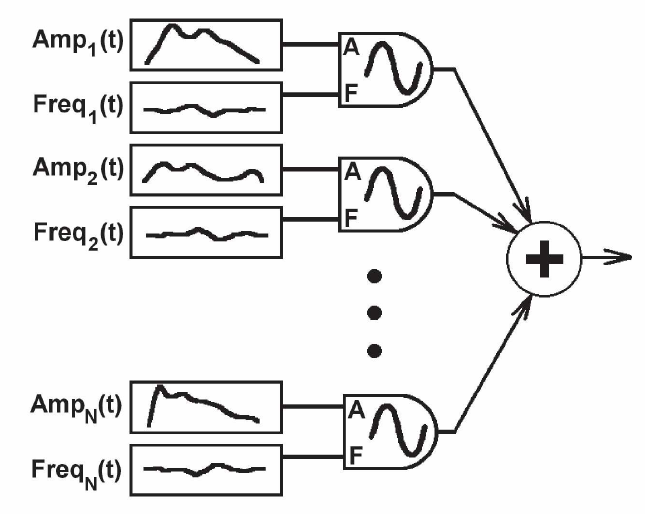
\includegraphics[width=0.5\textwidth]{sinusoidal_add_synth.PNG}
      \caption{Sinusoidal Additive Synthesis Algorithm \cite{Cook:2002:RSS:515316}.}
      \label{fig:sin_add_synth}
\end{figure}

\subsection{Filter-based Modal Synthesis}\label{sec:add_synth}

\paragraph{Band-pass Filters\\}\label{par:bpf}

At this point we will give some basic description of the band-pass filter since it is widely used in this thesis. Band-pass filters (BPFs) take a signal as input and give only a range of it as output, attenuating the rest of the frequencies. This range depends on the central frequency $f_c$. A filter of this kind is a result of a cascading of a low-pass and a high-pass filter circuit.

The passing range or ``band'' of frequencies is called \textbf{Bandwidth (BW)}. Defining as 0db the resonant peak, we can find the two cut-off frequencies ($f_{c{_\textsc{lower}}}$ and $f_{c_{\textsc{higher}}}$) at -3dB. The range between them is the bandwidth (equation \ref{eq:bw}). In figure \ref{fig:resp_bpf} we can see the frequency response of a BPF. \cite{bib:bpf}. 
\begin{equation}\label{eq:bw}
BW = f_{c_{\textsc{higher}}}-f_{c_{\textsc{lower}}}
\end{equation}   

\begin{figure}[H]
  \centering
    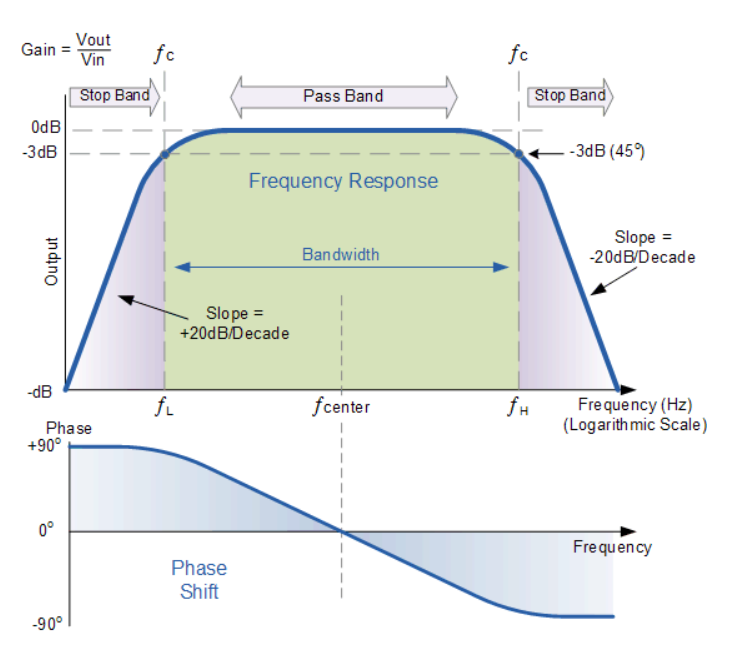
\includegraphics[width=0.7\textwidth]{BPF.PNG}
      \caption{Frequency Response of a Band-pass Filter  \cite{bib:bpf}.}
      \label{fig:resp_bpf}
\end{figure}

\paragraph{Synthesis\\}\label{par:synth}

This method is also additive, since we are adding the outputs of a number of band-pass filters. To synthesize a sound using this method, we use as many filters as the modal frequencies. The filter takes as input an impulse, the center frequency which is the modal frequency and a \textbf{Quality factor (Q-factor)} which specifies the bandwidth of the filter. The Q-factor is calculated heuristically, depending on the material of the sound and is inversely proportional to the bandwidth ($Q=f_c/BW$), so the lower the Q-factor, the wider the bandwidth and vice-versa. Hence, more and less frequencies respectively will be included in the \colorbox{pink}{audible} range. We call the above structure a \textit{resonator}, which also includes a multiplication with the corresponding amplitude, taken from the $A$ matrix.

\begin{figure}[H]
  \centering
    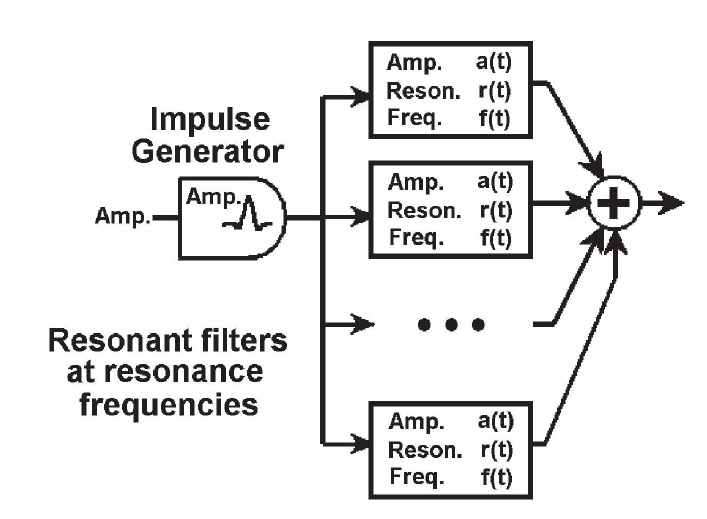
\includegraphics[width=0.5\textwidth]{filter-based_add_synth.PNG}
      \caption{Filter-based Modal Synthesis Algorithm \cite{Cook:2002:RSS:515316}.}
      \label{fig:filter_synth}
\end{figure}

\section{3D Audio}
In VR/AR applications, the location of the incoming sound plays as significant role as the sound itself. 


\chapter{Overview of Method and Tools Used}\label{ch:method}
%\section{Overview of the tool}
The aim of this thesis is to provide sound designers with an easy-to-use tool which enriches video games with procedural and physics-based audio instead of having to use prerecorded sounds. The tool enables to control contact sounds (impact, rolling and scratching) produced by vibrating objects through high level parameters that characterize the objects (size, material and surface roughness). The challenge is to offer realistic real-time and event-based sounds without high CPU usage.

\begin{figure}[H]
  \centering
    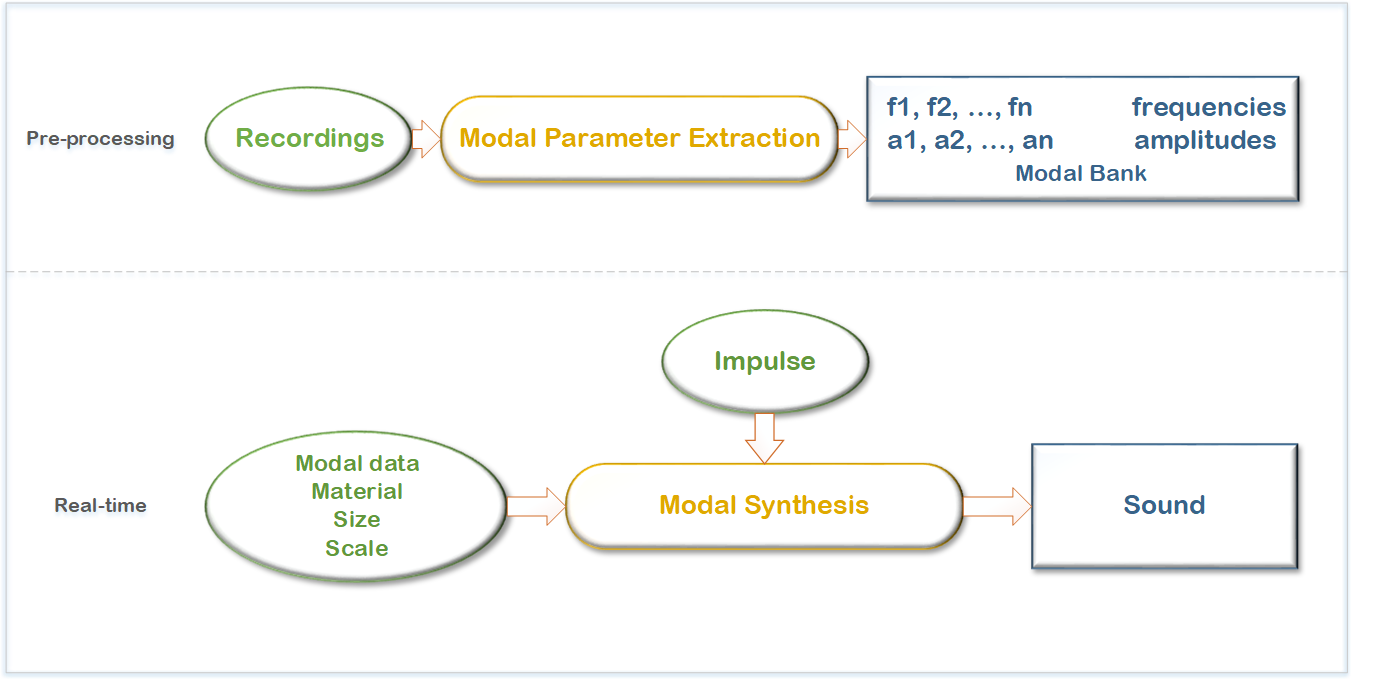
\includegraphics[width=\textwidth]{overview.png}
      \caption{Tool overview.}
      \label{fig:synth_proc}
\end{figure}

To create this tool, the procedure described in figure \ref{fig:synth_proc} was followed. To extract the modal parameters of vibrating objects the ``Example-guided'' method described in \ref{sec:exampleguided} was used due to its better integration within the audio pipeline as opposed to the rest of techniques presented in \ref{sec:modal_extraction}. The first step was to find several everyday objects that were made of different materials (plastic, wood, ceramic, glass and metal). This is because a priority in this thesis is the synthesis of sounds based on material properties. To obtain sound variations along the object's surface (see second method in \ref{sec:sound_variation}) the chosen objects were divided into areas that produced similar sounds when struck (e.g. bottle neck, rim of glass, etc). Between two and six sounds were recorded depending on the object. An example is presented in the following section for illustration \ref{sec:recordings}.

The recordings were then used to extract the data needed for the sound synthesis with the ChucK programming language. Some involved \gls{DSP} algorithms that employ the \gls{FFT} are used to capture the modal frequencies and gains specific of the object and which are present in the supplied audio clips. This process is explained in more depth in section \ref{sec:chuck}. 

As far as the modal synthesis of impact sounds is concerned, the two methods shown in \ref{sec:modal_synth} have been implemented into Pure Data patches \ref{sec:impact_synth} to evaluate differences between the output sounds. Scratching and rolling sounds (see \ref{sec:scratching_synth} and \ref{sec:rolling_synth} respectively) also make use of the filter-based method.

 At the same time, we made a 3D model of every object we used. We combined the 3D models with their corresponding data and the synthesis patches inside Unity\textsuperscript{\textregistered} software \cite{bib:unity}. At this point, the frequencies and amplitudes corresponding to the point of collision are assigned to the patch. The sound is then sent to the audio DSP chain and is played back. 

\section{Recordings}
The first step of this tool creation is to obtain the necessary data for audio synthesis. Thus, we performed recordings of the sound produced of the object when being hit in several areas. The signal of those recordings was used to extract the modal frequencies and their peaks. 

Since we only used simple shape everyday objects, we could easily assume that nearby points produce almost the same sound and thus separate the object into ``sound areas'' instead of calculating different modal matrices for each vertex. Unofficial tests proved that this accuracy-computational complexity trade-off was acceptable. A sample object and its division in areas is shown in figure \ref{fig:pot_sep}.

\begin{figure}[H]
  \centering
    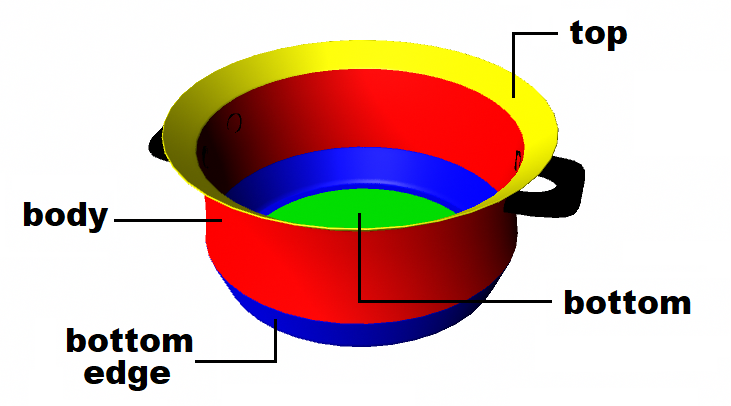
\includegraphics[width=0.6\textwidth]{potseparated.png}
      \caption{Division of an object into areas with similar sound.}
      \label{fig:pot_sep}
\end{figure} 

The procedure of the recordings will be explained in detail in section \ref{sec:recordings}.

The reason why we chose to extract the modal data from recordings instead of using the FEM method as in \cite{director2001synthesizing} or \cite{o2002synthesizing} or using spring-mass systems as in \cite{raghuvanshi2006interactive} lays in simplicity. More specifically, recordings of impact sounds is much easier for our target users to perform, if they want to extend our tool, than having to use complex calculations or software.

\section{3D models}
To achieve realistic sounds, we have to correspond the impact recordings of the real objects with same size 3D models of them. Hence, we measured the dimensions and weight of the eleven objects and used those data to model the objects. In table \ref{tab:dim_weig} the maximum dimensions and the weight of the objects are displayed. To create the 3D models of the objects we used \textbf{Maya Autodesk} software \cite{bib:maya} and exported them as FBX\textsuperscript\textregistered\ files \cite{bib:fbx} which is a format recognizable by Unity\textsuperscript{\textregistered}.

\begin{table}[H]
	\centering
    \begin{tabular}{ l c r c}
    \toprule
    \textbf{Name} & \textbf{Dimensions(cm)} & \textbf{Weight(g)} & \textbf{Picture} \\
    \toprule 
    Cooking pot & $21.5L\times 21.5W\times 10.8H$ & 680 & 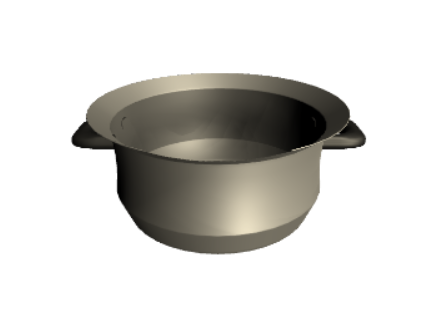
\includegraphics[scale=0.1]{3DmodelsPics/cp.PNG} \\ 
    Cup & $7.5L\times 7.5W\times 6H$ & 125 & 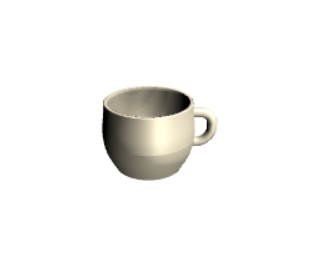
\includegraphics[scale=0.1]{3DmodelsPics/cup.PNG} \\ 
    Cutting board & $41.5L\times 26.5W\times 4.5H$ & 2200 & 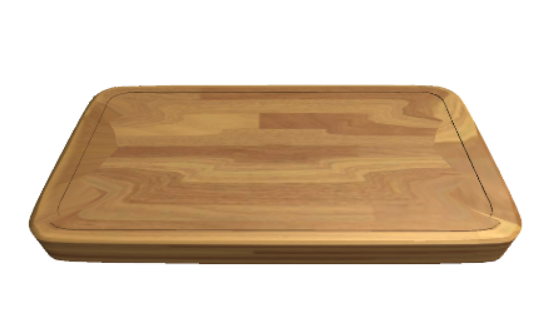
\includegraphics[scale=0.1]{3DmodelsPics/cb.PNG} \\ 
    Jug & $14L\times 10W\times 21.5H$ & 150 & 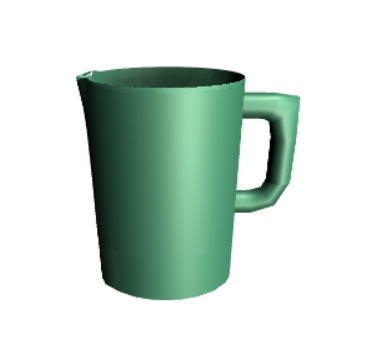
\includegraphics[scale=0.1]{3DmodelsPics/jug.PNG} \\ 
    Mortar & $11L\times 11W\times 19H$ & 850 & 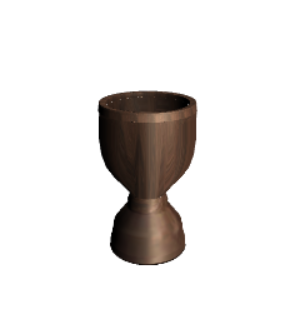
\includegraphics[scale=0.1]{3DmodelsPics/mortar.PNG} \\
    Bowl & $20L\times 20W\times 10.5H$ & 100 & 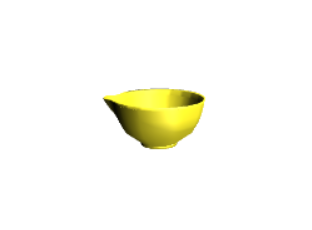
\includegraphics[scale=0.1]{3DmodelsPics/bowl.PNG} \\
    Plate & $25.5L\times 25.5W\times 2.5H$ & 700 & 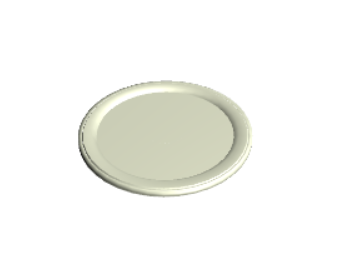
\includegraphics[scale=0.1]{3DmodelsPics/plate.PNG} \\
    Rolling pin & $43L\times 7W\times 7H$ & 700 & 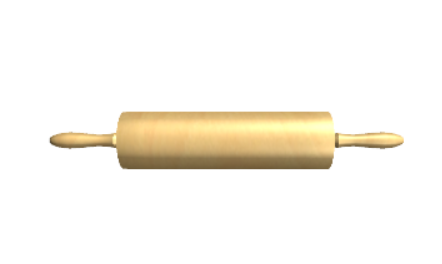
\includegraphics[scale=0.1]{3DmodelsPics/rp.PNG} \\
    Wine bottle & $7L\times 7W\times 29H$ & 400 & 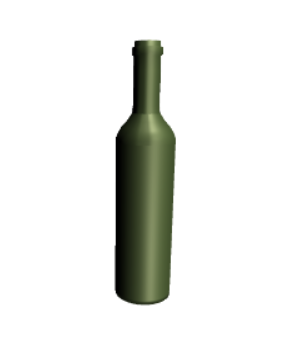
\includegraphics[scale=0.1]{3DmodelsPics/bottle.PNG} \\
    Wine glass & $8L\times 8W\times 18H$ & 120 & 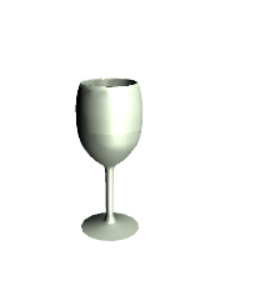
\includegraphics[scale=0.1]{3DmodelsPics/glass.PNG} \\
    Wok & $35L\times 35W\times 9.5H$ & 1225 & 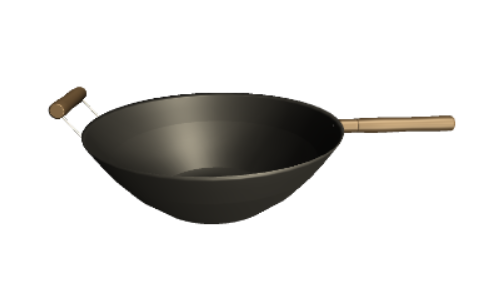
\includegraphics[scale=0.1]{3DmodelsPics/wok.PNG} \\
    \bottomrule
    \end{tabular}
    \caption{Maximun dimensions and weight of the eleven objects.}
    \label{tab:dim_weig}
\end{table}

%     \begin{minipage}{.45\textwidth}
%      \begin{itemize}
%        \item Cooking Pot
%		\item Cup
%		\item Cutting Board
%		\item Jug
%		\item Mortar
%		\item Bowl
%		\item Plate
%		\item Rolling Pin
%		\item Wine Bottle
%		\item Wine Glass
%		\item Wok
%     \end{itemize}
%  \end{minipage}
%    \begin{minipage}{.45\textwidth}
%    	\hspace{-3cm}
%    		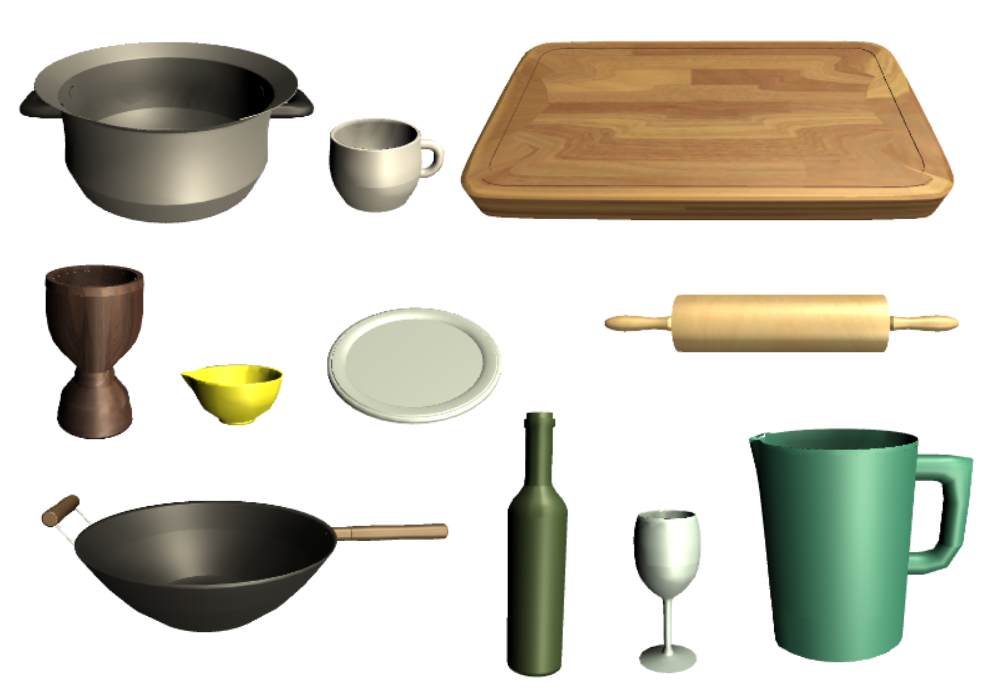
\includegraphics[scale=0.4]{3DmodelsPics/3dmodels.png}
%     		 \label{fig:3d_all}
%    \end{minipage}

\section{Modal data extraction}\label{sec:chuck}
\textbf{Chuck} language is a music programming language, made for ``real-time sound synthesis and music creation'' as mentioned in their website \cite{bib:chuck}. It's biggest advantage is the way it manipulates time. More specifically, the user specifies how long a sound will last, independent of other sounds that may play at the same time.

We used the ChucK language at the starting point of our thesis to identify and extract the peaks of the recorded audio files. The algorithm used in this part of the thesis is made by Perry Cook for the course \textbf{``Physics-Based Sound Synthesis for Games and Interactive Systems''} held by \textit{Perry Cook} and \textit{Julius O. Smith} at \textbf{Kadenze Academy} \cite{bib:physicsbasedcourse}.

From a modal analysis one can find out that each object vibrates in a very high number of modes. Although, most of them are inaudible and do not contribute to the sound model. It is, therefore, desirable to preserve CPU cycles by reducing the number of calculated modes. Based on the recommendations of the author Perry Cook, we chose ten as the sufficient amount of modes for the analysis/synthesis.  Afterwards, the algorithm having taken a recording as input, computes its histogram and identifies its peaks. The frequencies where peaks occur are the modal frequencies candidates. Depending on the numbers of peaks we chose, the algorithm outputs the strongest peaks. Finally, the algorithm finds the maximum value of the signal on each peak, calculating the corresponding amplitude of each mode.

ChucK language was chosen, because of its build-in functions to manipulate sound like \textit{Fast Fourier Transform (FFT)} of input audio samples and windows functions \cite{bib:chuck_doc}. Another option to extract the peaks of the sound waves could be to use python programming language on audio files, but this would request to program a number of functions or include a number of libraries that perform actions like file input/output, FFT and more. 

\Todo{should we explain why we used FFT?} 
 
\section{Modal synthesis patches}
\textbf{Pure Data (Pd)} is another music programming language. It is open source and the main difference from ChucK language is that Pd is a visual or ``patcher'' programming language, using objects instead of code, linked together to form a sequence \cite{bib:pd}. We chose to use this software as our synthesis engine mainly because of the ability to compile the patches into C\# code, as explained below in section \ref{sec:heavy}. Another important reason for choosing it is the possibility of real-time parameter manipulation and easy testing during implementation period.

All synthesized sounds (impact, rolling and scratching) are being synthesized under one main pd patch. However, two different patches have been developed, one for each of the two examined methods. Since the audio synthesis patch takes the modal data as input, every object can use the same patch. The synthesis patches will be described in detail in section \ref{sec:synthesis_implem}.

%For optimization reasons, we lowered the number of modes down to 10 instead of 20 that we initially had, since the extra 10 did not add any useful information to the output sound. In addition, we clipped the range of frequencies to the human audible range of 20Hz to 20KHz. 

\Todo{develop more?}

\section{Heavy Compiler}\label{sec:heavy}
\textbf{Heavy} is a compiler that generates audio plugins from Pd patches in interactive sound and music applications \cite{bib:heavy}. In this thesis we used it to compile Pd patches into Unity\textsuperscript{\textregistered} audio plugins. Heavy's interface is their website where users upload patches and then are able to download the corresponding plugins and put them into their applications. The plugins we used consist of DLL files and a C\# (Unity\textsuperscript{\textregistered} code) script that allows communication of the plugins with the rest of the scripts and also enables the sound card to play audio.

Through the generated C\# script, we are able to send float values to the audio plugins - which are the compiled Pd patches - as inputs to generate the appropriate sound. Those floats are the frequencies and their corresponding amplitudes, the quality factor (Q-factor) of the band-pass filters, the impact force of the collision, the roughness of the object, the multiplier of the size of the object, the velocity of the object and the rolling and scratching duration times. A difficulty we encountered by using this compiler was the inability of sending a whole array or list of floats. Thus, we had to send every frequency and every amplitude individually, creating a float parameter for each.
 
\subsection{Why not OSC?}
The most popular way to communicate between Unity\textsuperscript{\textregistered} and Pure Data is the Open Sound Control (OSC) protocol. The reason why we did not use it is because it requires establishing a connection between two software programs and send data between them. On the other hand, Heavy makes everything work inside Unity\textsuperscript{\textregistered} and it is as simple as passing floats between scripts. 

\section{Unity\textsuperscript{\textregistered}}
\textbf{Unity\textsuperscript{\textregistered}} is a game engine software. This is where all previous work is combined together and outputs the final product. For the purpose of this thesis, several demonstration scenes are made inside Unity\textsuperscript{\textregistered} where objects are struck in several points and produce different sounds. 

The first part of the Unity\textsuperscript{\textregistered} implementation is the assignment of modal data to every different area of the object. This is done in linear time ($O(n)$ for $n$ modes). The whole procedure of assigning the appropriate data includes the identification of the area of the object that collided, filling the arrays with the corresponding data and set the parameters of the plugins. Afterwards, the type of collision is identified and a number of other parameters are calculated and sent to the plugins, like the impact force and the duration of the collision.

Audio in Unity\textsuperscript{\textregistered} is enabled using the \textit{OnAudioFilterRead()} function. This function is running in the audio thread, which is a different one from the main thread. Its job is to send the audio buffer to the sound card and is called every $\sim 20$ms, so it does not require a function call from the programmer \cite{bib:unity_doc}.

\section{Microsoft Hololens Emulator}
\Todo{keep it or not?}


\chapter{Results \& Discussion}\label{ch:results}


\section{Which Synthesis Method Is Better?}

\section{Did we manage to achieve what we wanted?}

\section{How can we improve our work?}
\include{discussion}
\chapter{Conclusion}

A sound designing tool has been presented in this study, where two different synthesis algorithms are implemented. The goal is to achieve physics-based procedural audio implemented in a virtual environment using the Unity\textsuperscript{\textregistered} game engine. 

A number of everyday objects which are separated into different ``sound areas'' are recorded by striking each one of them at these different surface location. 3D models of these objects are created, matching their shape and dimensions. By analyzing the recordings with \gls{DSP} audio algorithms, it is possible to extract the modal data necessary for the sound synthesis stage. This data is fed into the modal synthesis model which is driven by physics events from the game engine. This process transfers successfully the sound properties of the real world objects to their corresponding virtual ones but has some limitations. Further extension of the tool is possible by adding more types of objects while following the same procedure.

Three different kind of contact sounds have been synthesized; impact sounds and continuous contact sounds, namely rolling and scratching. The tool's \gls{UI}, with high level adjustable parameters, enables the designers to customize the sounds according to their needs. A metallic object can be transformed into a wooden one just by adjusting a slider. In addition, having the original objects' sizes as reference, designers are able to scale the produced sound together with the object. Finally, the surface's roughness can be fine-tuned to match the desired sound of a rolling object.

Listening experiments performed to several individuals did not favor noticeably one synthesis method over the other. The methods presented better results for certain materials and \textit{vice versa}. Furthermore, it was proven that sound variation along an object's surface is desirable and is preferred over just a single sound per object. Finally, the distinction of the different materials for a range of values of the Q-factor was identified well from the participants. Hence, the use of a 1D slider to shift from one material to another was justified.

Although the extraction of data from recordings offers computational efficiency, it is impossible to include the whole sound information without alterations. Thus, the synthesized sounds do not sound exactly like the reference ones, but their source is highly recognizable. In addition, the tool used for striking the objects produces a sound as well, which interferes with the desired sound. Another aspect that can improve the recording process is to try to approximate as much as possible the system to a free vibration when holding the struck object in the air.

Physics-based procedural audio aims to increase realism and sense of presence in virtual worlds. Audio events match exactly with graphic events and complement one another, producing a compelling experience for the user.
\bibliographystyle{plain} % pr�v ogs�: is-unsrt, alpha, plain
\bibliography{biblio/template-bib}
\nocite{*} % \nocite bruges til b�ger som skal med i litteraturlisten
%             men som ikke er refereret til. Alts� baggrundsstof mv.


% \appendix % Alphabetic chapter numbering
% \renewcommand{\appendixtocname}{Appendix} % Change appendix name for the table od contents
% \addappheadtotoc % 'Appendix' to the table of contents
\appendix

\chapter{Pure Data Patches}\label{ap:pd_patches}
\Todo{make the patches more readable and replace the pics}

\section{Filter Based Additive Synthesis}
\begin{figure}[H]
  \centering
    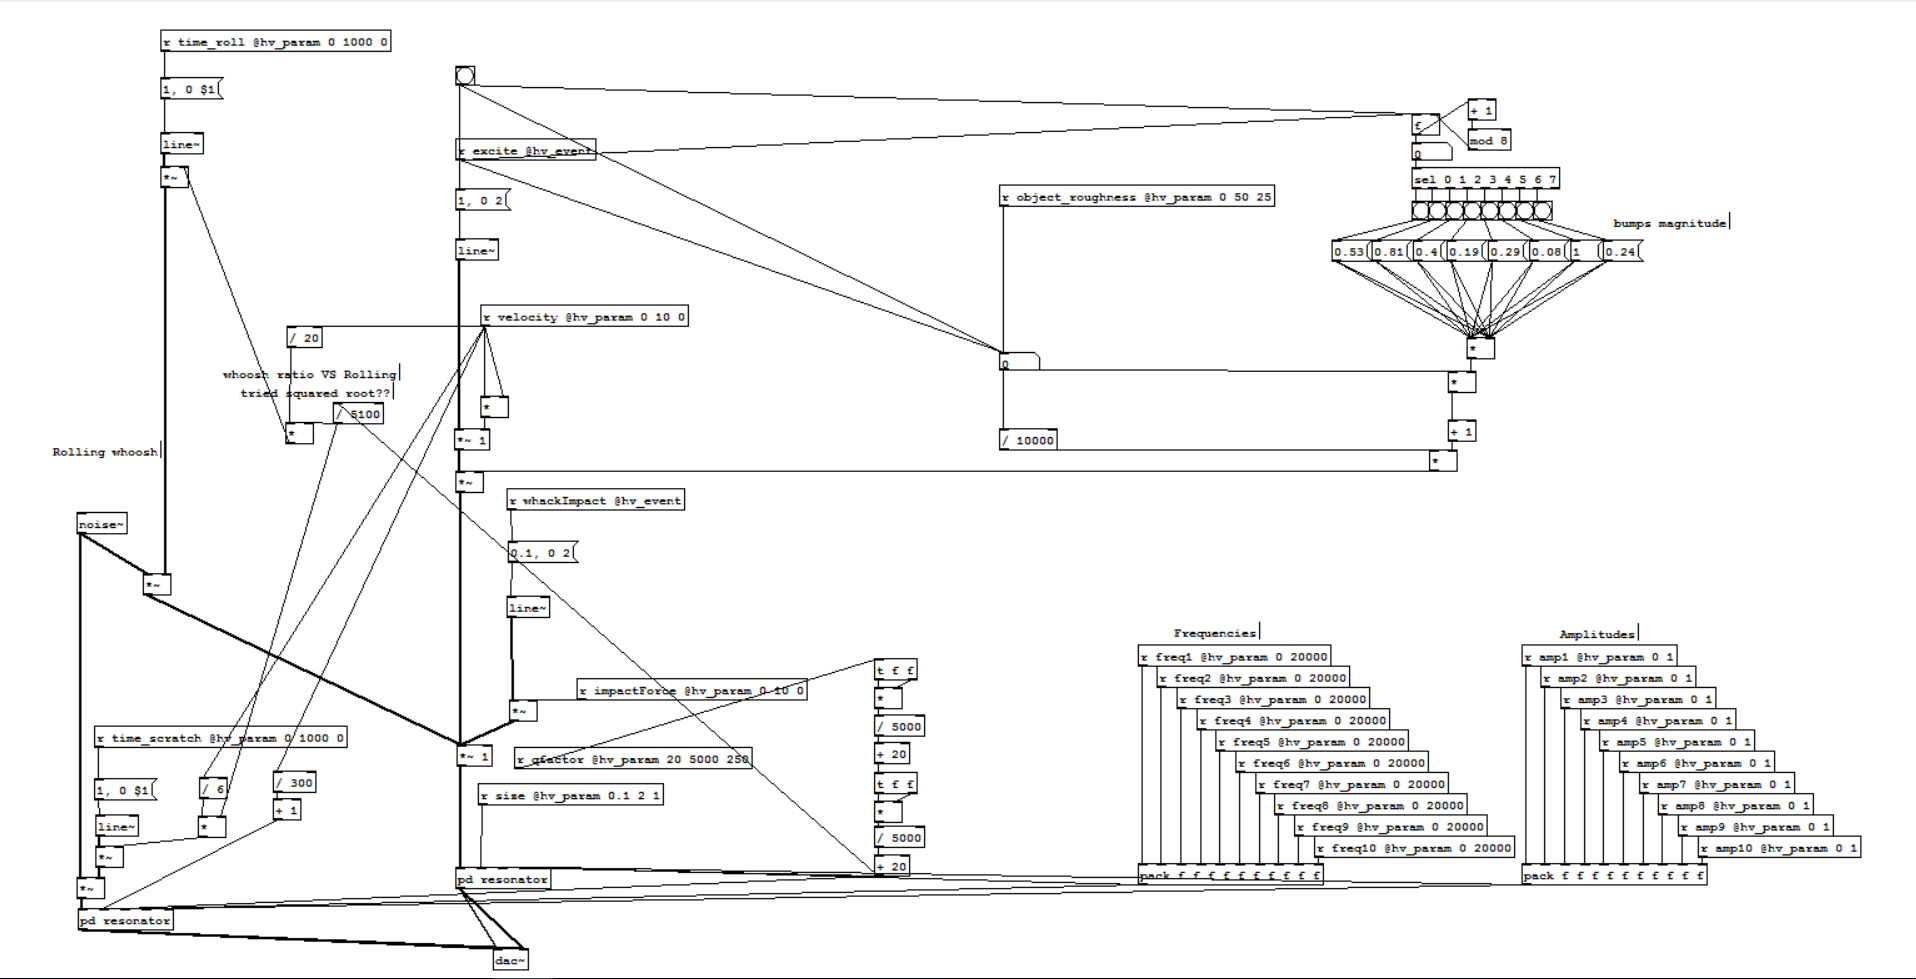
\includegraphics[width=\textwidth]{PdPatches/FBmain.PNG}
      \caption{The main Pure Data patch for the filter-based additive synthesis.}
      \label{fig:FBmain}
\end{figure}

\begin{figure}[H]
  \centering
    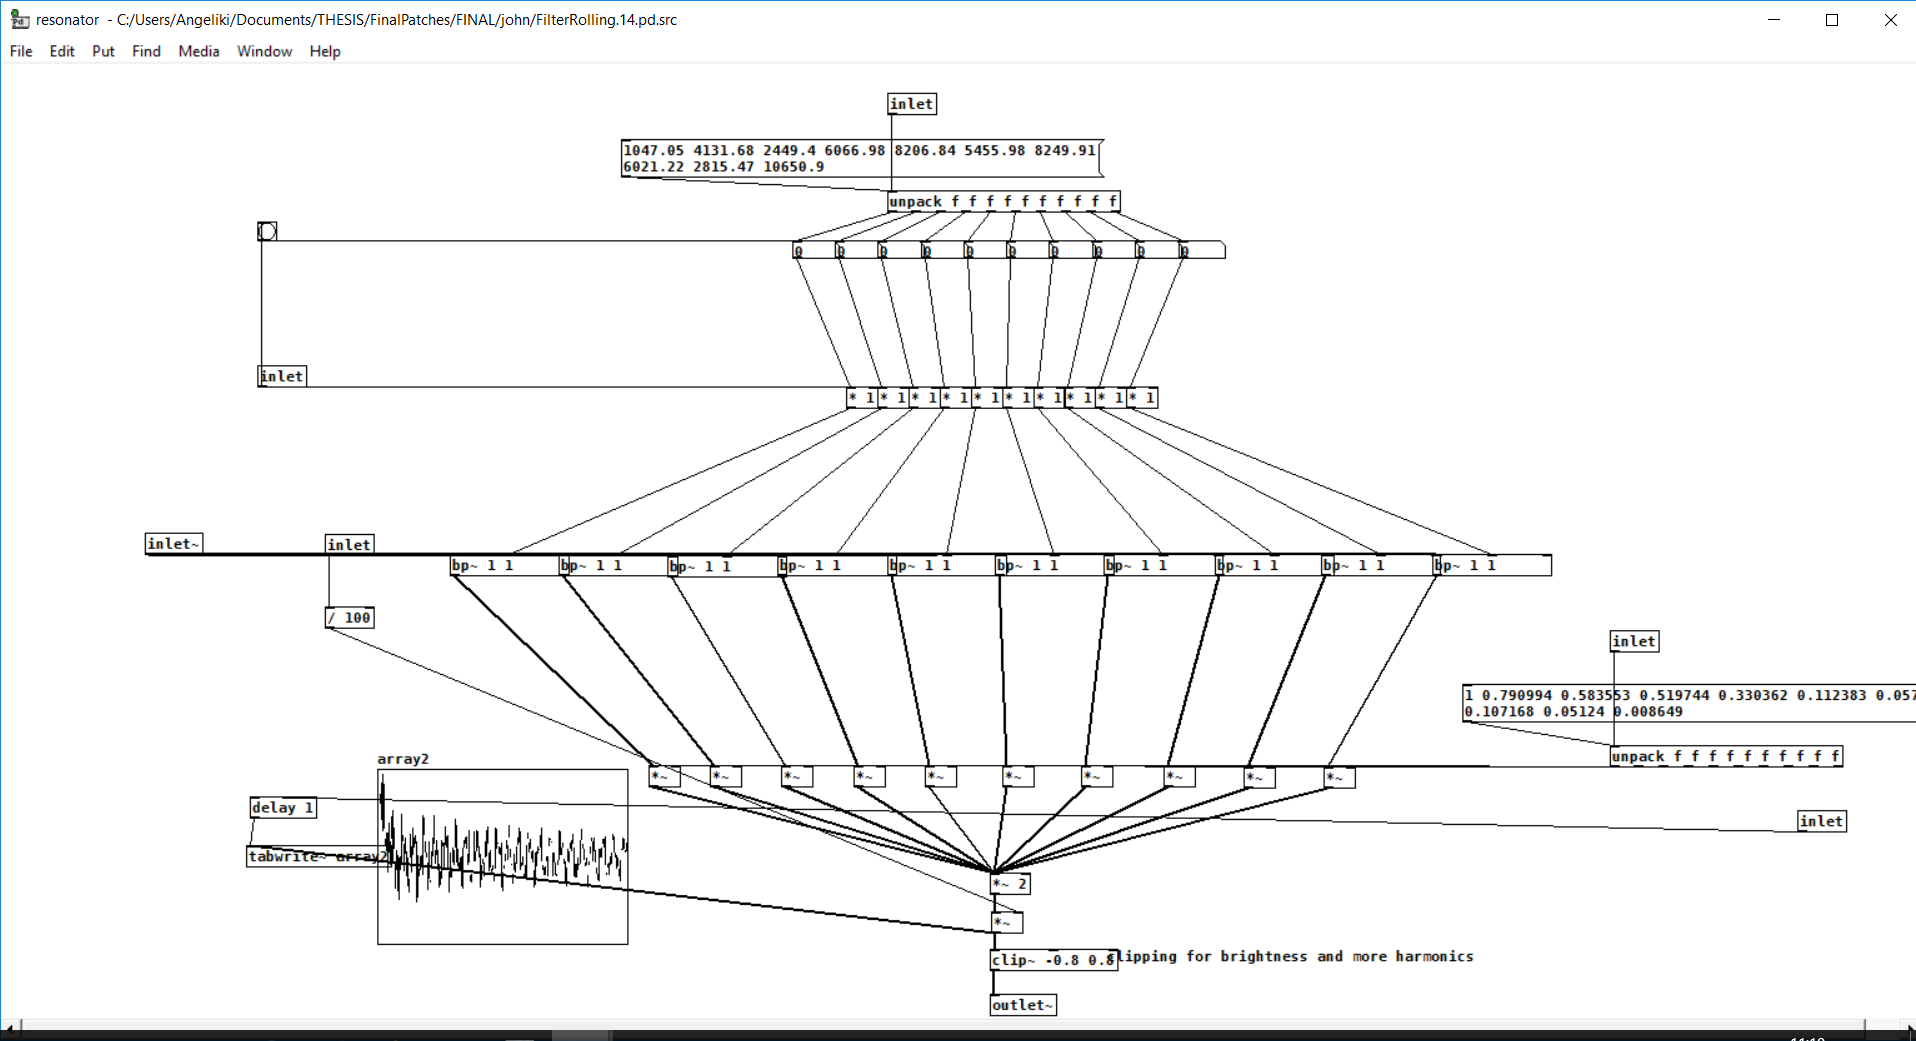
\includegraphics[width=\textwidth]{PdPatches/FBresonator.PNG}
      \caption{The resonator Pure Data patch for the filter-based additive synthesis.}
      \label{fig:FBres}
\end{figure}

\section{Sinusoidal Additive Synthesis}

\begin{figure}[H]
  \centering
    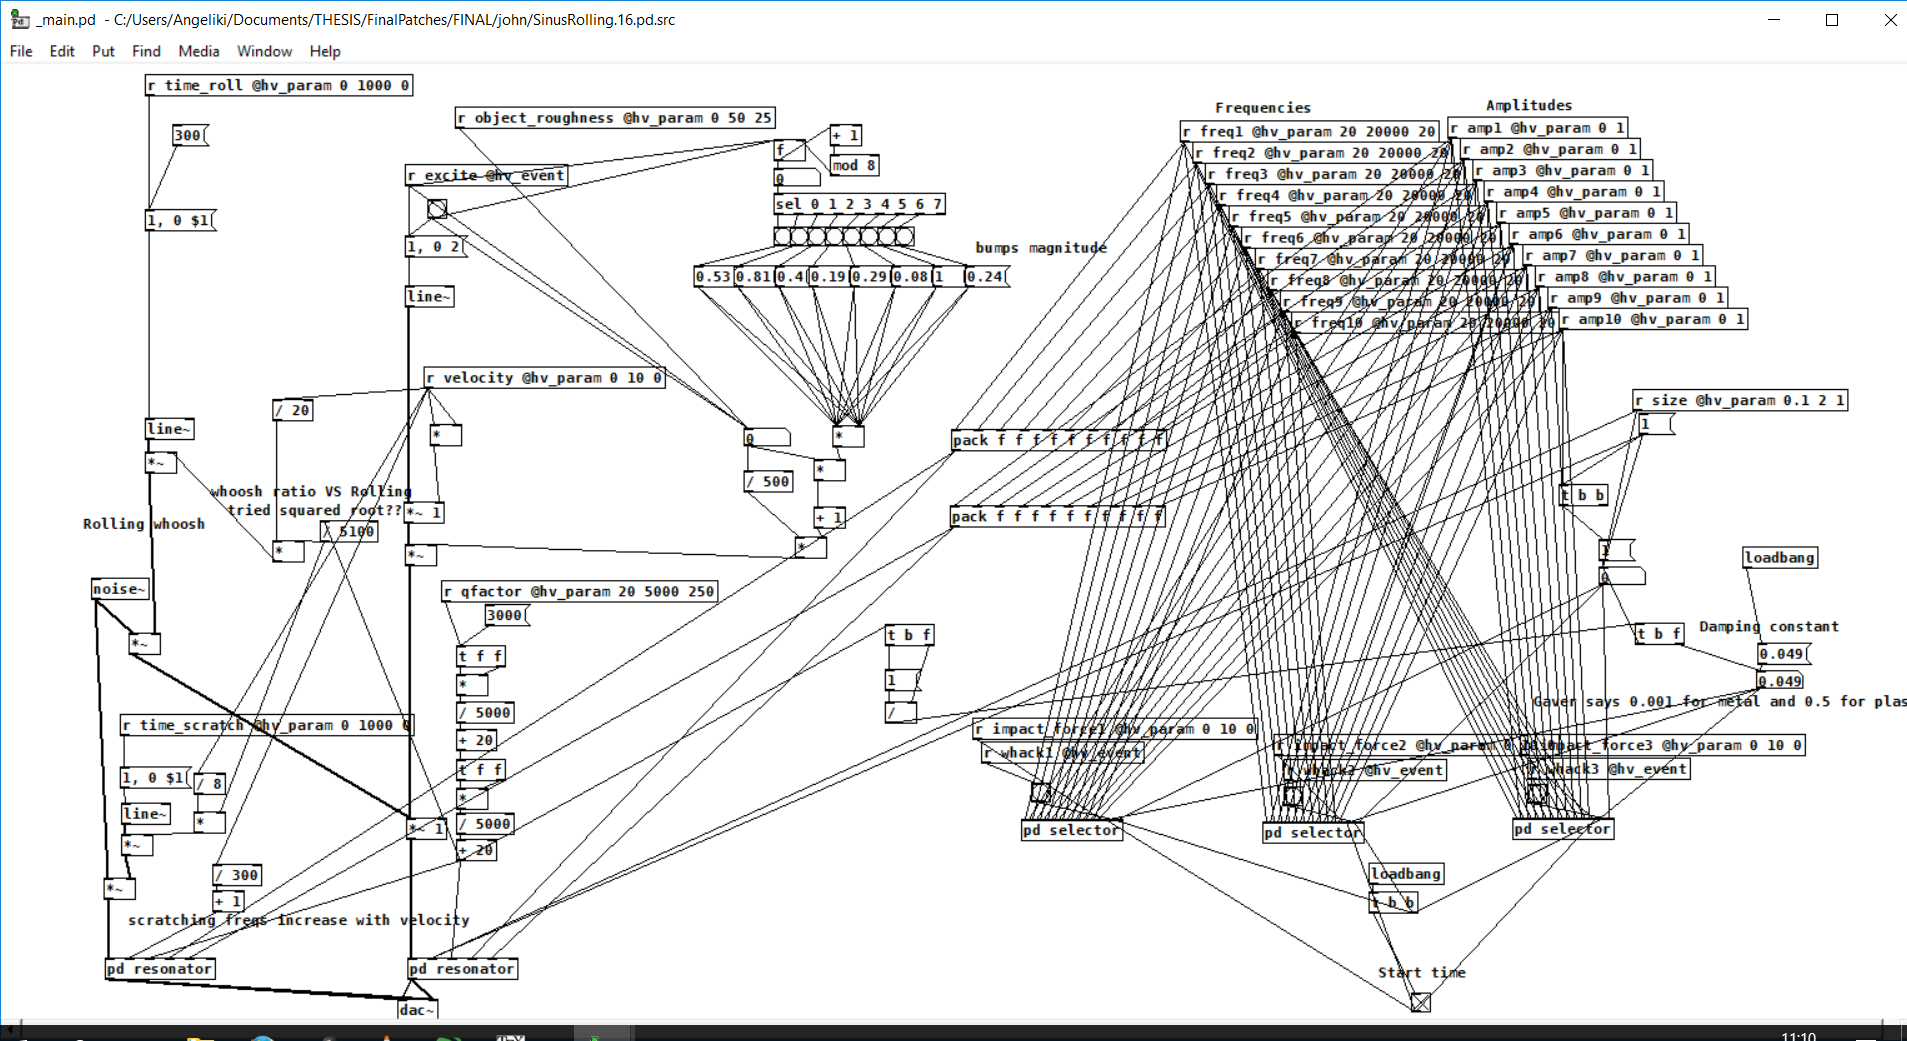
\includegraphics[width=\textwidth]{PdPatches/Smain.PNG}
      \caption{The main Pure Data patch for the sinusoidal additive synthesis.}
      \label{fig:Smain}
\end{figure}

\begin{figure}[H]
  \centering
    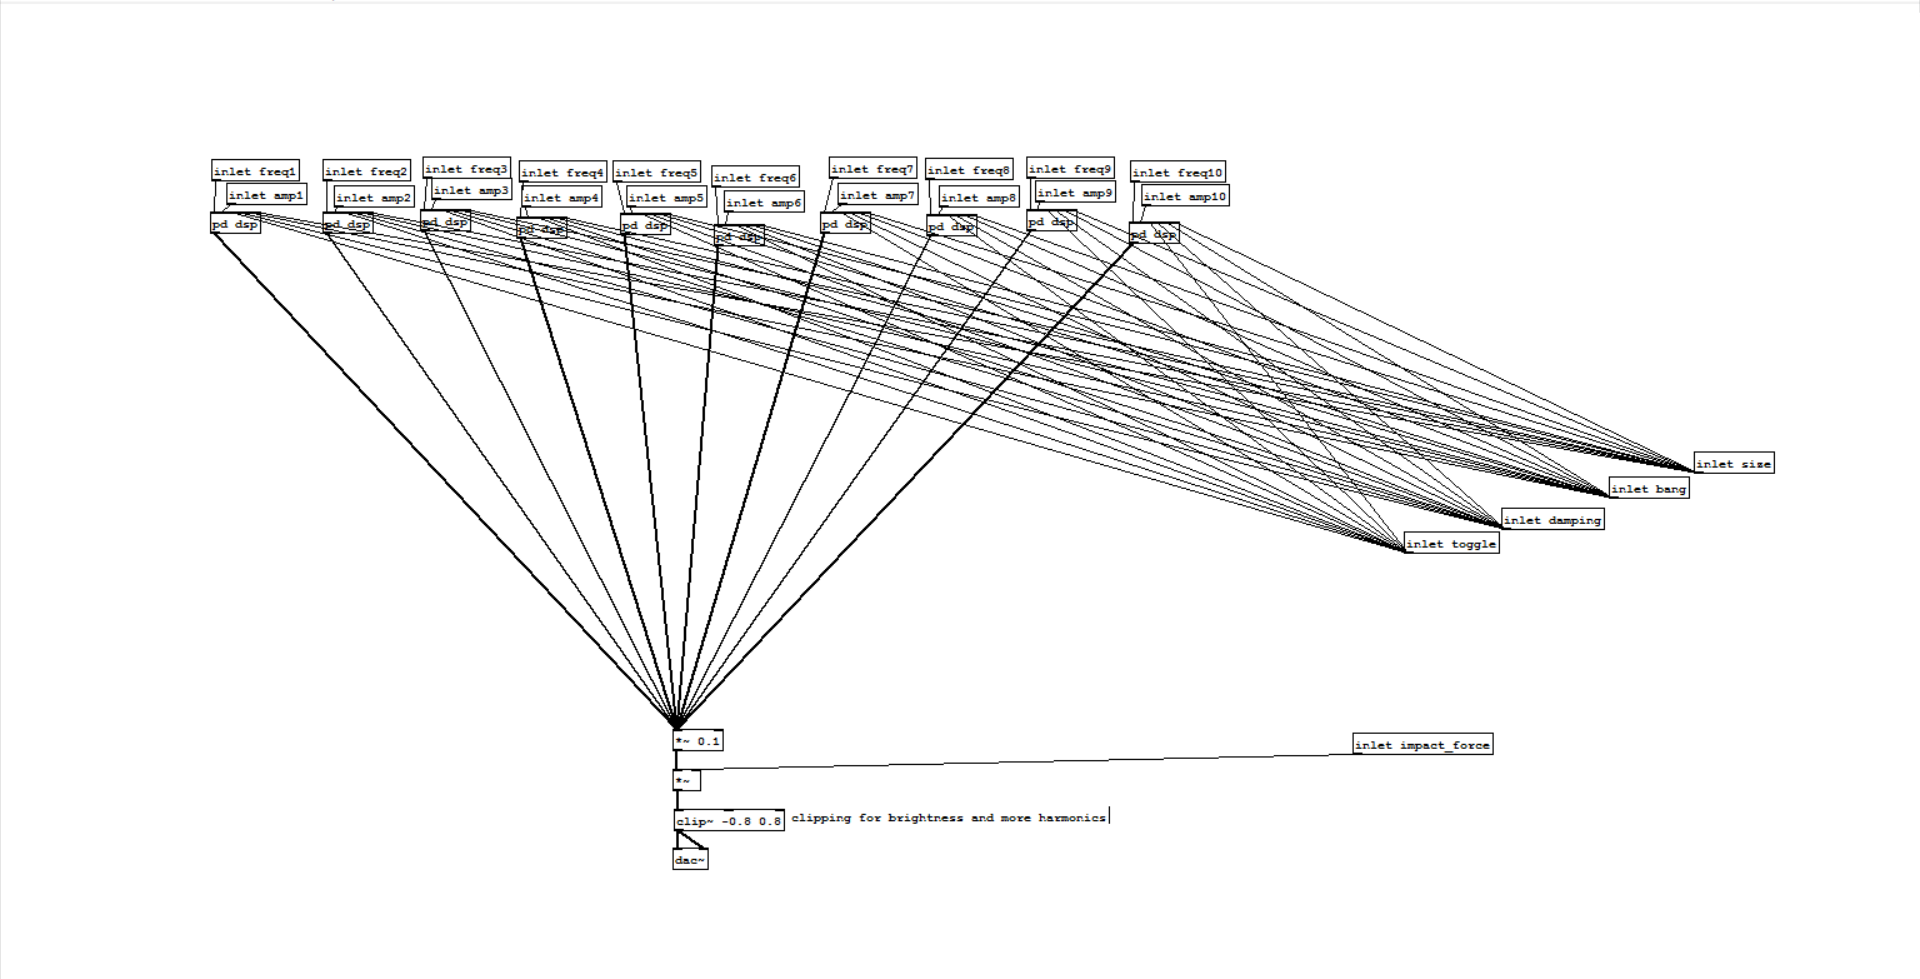
\includegraphics[width=\textwidth]{PdPatches/Sselector.PNG}
      \caption{The selector Pure Data patch for the filter-based additive synthesis.}
      \label{fig:Ssel}
\end{figure}

\begin{figure}[H]
  \centering
    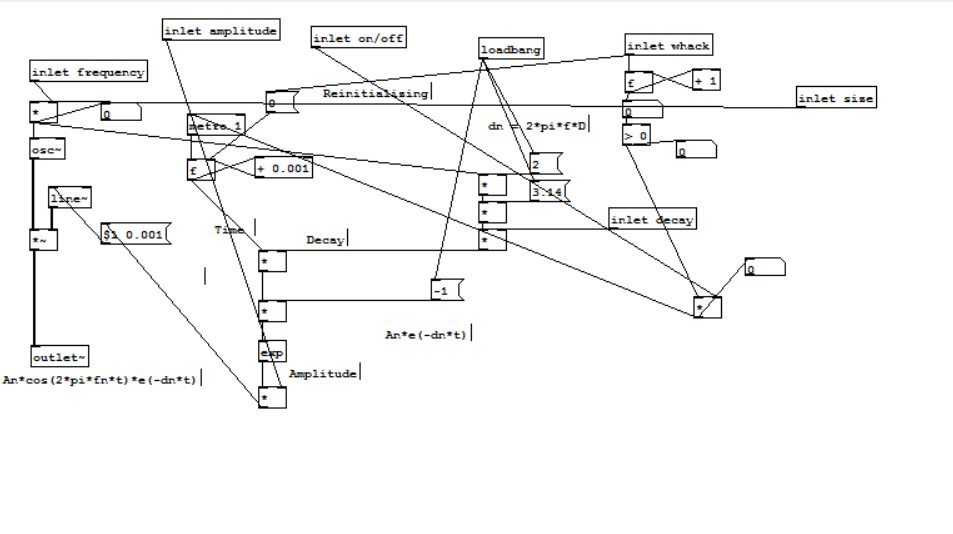
\includegraphics[width=\textwidth]{PdPatches/Sdsp.PNG}
      \caption{The dsp Pure Data patch for the filter-based additive synthesis.}
      \label{fig:Sdsp}
\end{figure}

\chapter{Spectrograms}\label{ap:spectrograms}
\section*{Plastic bowl}

\begin{figure}[H]
    \centering
    \begin{subfigure}[b]{0.25\textwidth}
        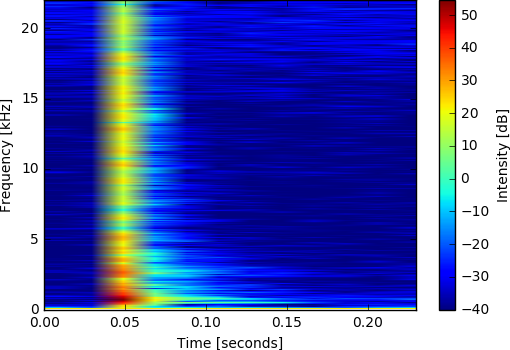
\includegraphics[width=\textwidth]{specs/spectrograms/plasticbowlTOP_rec.png}
    \end{subfigure}%
    ~ %add desired spacing between images, e. g. ~, \quad, \qquad, \hfill etc. 
      %(or a blank line to force the subfigure onto a new line)
    \begin{subfigure}[b]{0.25\textwidth}
        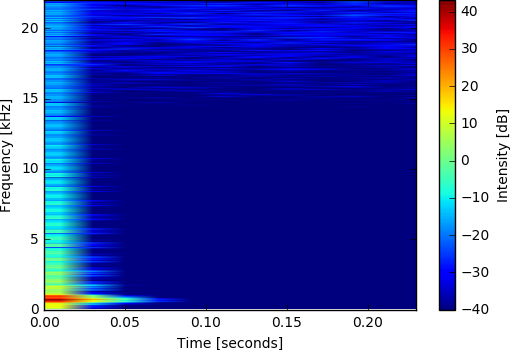
\includegraphics[width=\textwidth]{specs/spectrograms/plasticbowlTOP_sin.png}
    \end{subfigure}%
    ~ %add desired spacing between images, e. g. ~, \quad, \qquad, \hfill etc. 
      %(or a blank line to force the subfigure onto a new line)
    \begin{subfigure}[b]{0.25\textwidth}
        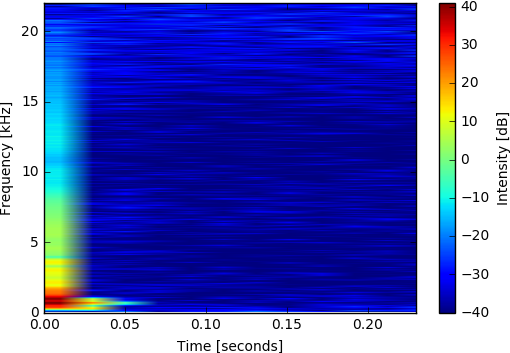
\includegraphics[width=\textwidth]{specs/spectrograms/plasticbowlTOP_fb.png}
    \end{subfigure}%
    %add desired spacing between images, e. g. ~, \quad, \qquad, \hfill etc. 
      %(or a blank line to force the subfigure onto a new line)
      
    \begin{subfigure}[b]{0.25\textwidth}
        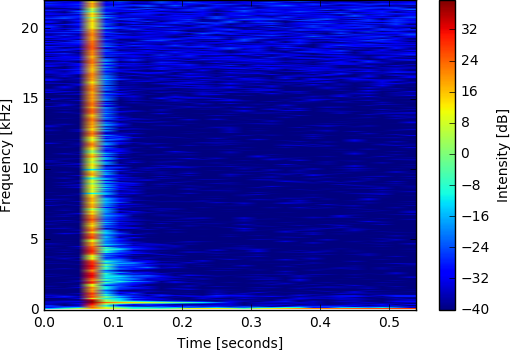
\includegraphics[width=\textwidth]{specs/spectrograms/plasticbowlBODY_rec.png}
    \end{subfigure}%
    ~ %add desired spacing between images, e. g. ~, \quad, \qquad, \hfill etc. 
      %(or a blank line to force the subfigure onto a new line)
    \begin{subfigure}[b]{0.25\textwidth}
        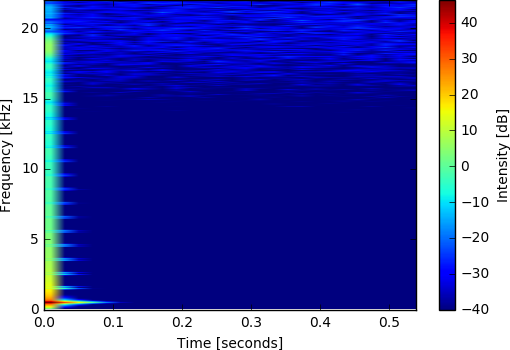
\includegraphics[width=\textwidth]{specs/spectrograms/plasticbowlBODY_sin.png}
    \end{subfigure}%
    ~ %add desired spacing between images, e. g. ~, \quad, \qquad, \hfill etc. 
      %(or a blank line to force the subfigure onto a new line)
    \begin{subfigure}[b]{0.25\textwidth}
        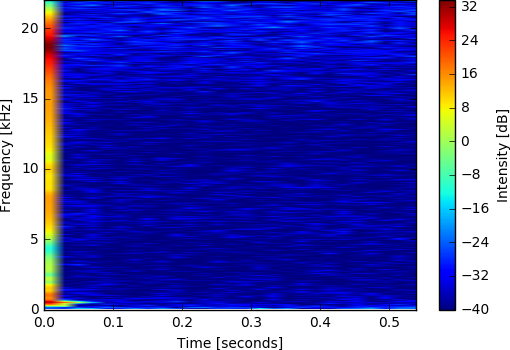
\includegraphics[width=\textwidth]{specs/spectrograms/plasticbowlBODY_fb.png}
    \end{subfigure}%
    %add desired spacing between images, e. g. ~, \quad, \qquad, \hfill etc. 
      %(or a blank line to force the subfigure onto a new line)
      
    \begin{subfigure}[b]{0.25\textwidth}
        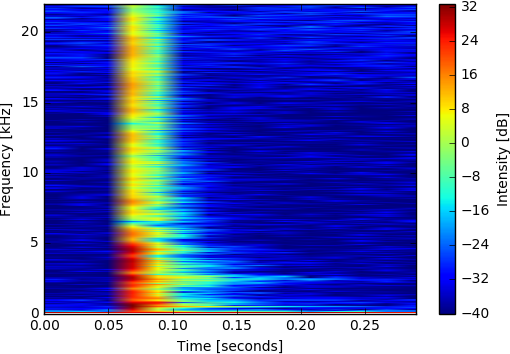
\includegraphics[width=\textwidth]{specs/spectrograms/plasticbowlBOTTOM_rec.png}
    \end{subfigure}%
    ~ %add desired spacing between images, e. g. ~, \quad, \qquad, \hfill etc. 
      %(or a blank line to force the subfigure onto a new line)
    \begin{subfigure}[b]{0.25\textwidth}
        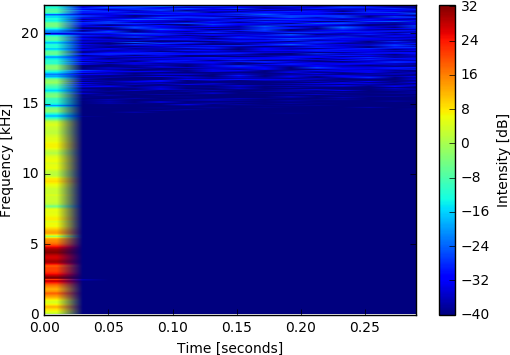
\includegraphics[width=\textwidth]{specs/spectrograms/plasticbowlBOTTOM_sin.png}
    \end{subfigure}%
    ~ %add desired spacing between images, e. g. ~, \quad, \qquad, \hfill etc. 
      %(or a blank line to force the subfigure onto a new line)
    \begin{subfigure}[b]{0.25\textwidth}
        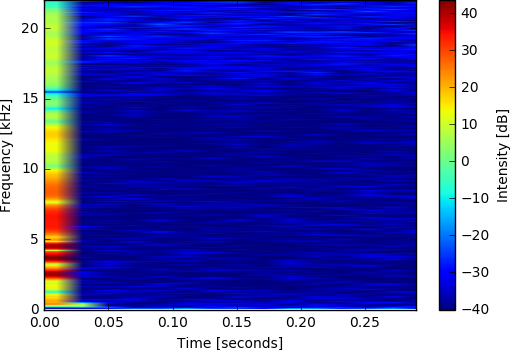
\includegraphics[width=\textwidth]{specs/spectrograms/plasticbowlBOTTOM_fb.png}
    \end{subfigure}%
\end{figure}

\section*{Wooden mortar}

\begin{figure}[H]
    \centering
    \begin{subfigure}[b]{0.25\textwidth}
        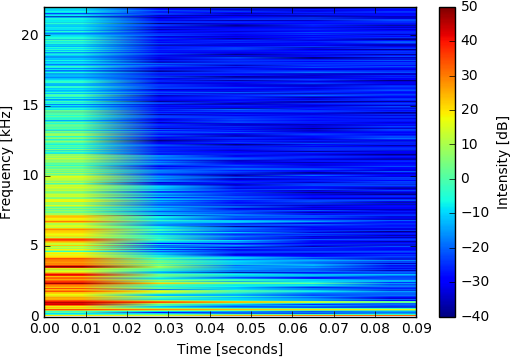
\includegraphics[width=\textwidth]{specs/spectrograms/mortarTOP_rec.png}
    \end{subfigure}%
    ~ %add desired spacing between images, e. g. ~, \quad, \qquad, \hfill etc. 
      %(or a blank line to force the subfigure onto a new line)
    \begin{subfigure}[b]{0.25\textwidth}
        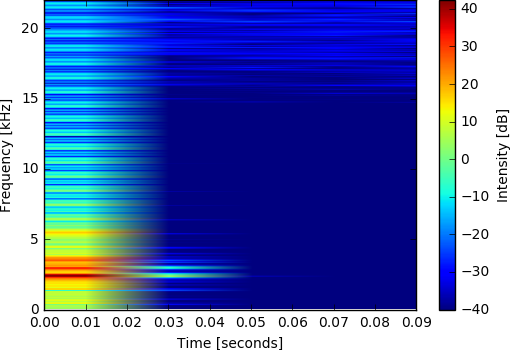
\includegraphics[width=\textwidth]{specs/spectrograms/mortarTOP_sin.png}
    \end{subfigure}%
    ~ %add desired spacing between images, e. g. ~, \quad, \qquad, \hfill etc. 
      %(or a blank line to force the subfigure onto a new line)
    \begin{subfigure}[b]{0.25\textwidth}
        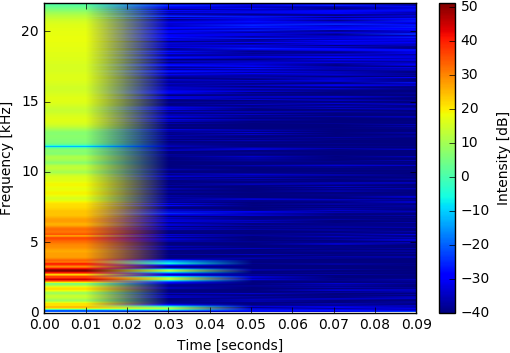
\includegraphics[width=\textwidth]{specs/spectrograms/mortarTOP_fb.png}
    \end{subfigure}%
    %add desired spacing between images, e. g. ~, \quad, \qquad, \hfill etc. 
      %(or a blank line to force the subfigure onto a new line)
      
    \begin{subfigure}[b]{0.25\textwidth}
        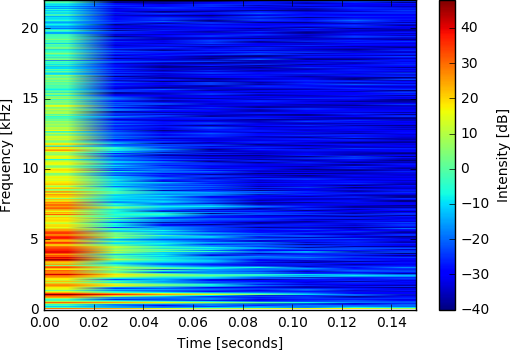
\includegraphics[width=\textwidth]{specs/spectrograms/mortarBODYUPPER_rec.png}
    \end{subfigure}%
    ~ %add desired spacing between images, e. g. ~, \quad, \qquad, \hfill etc. 
      %(or a blank line to force the subfigure onto a new line)
    \begin{subfigure}[b]{0.25\textwidth}
        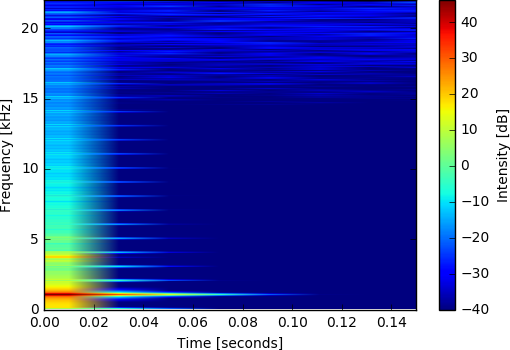
\includegraphics[width=\textwidth]{specs/spectrograms/mortarBODYUPPER_sin.png}
    \end{subfigure}%
    ~ %add desired spacing between images, e. g. ~, \quad, \qquad, \hfill etc. 
      %(or a blank line to force the subfigure onto a new line)
    \begin{subfigure}[b]{0.25\textwidth}
        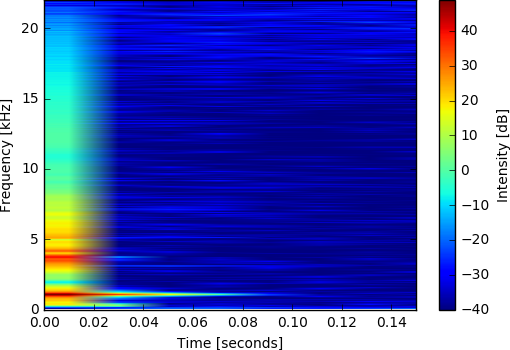
\includegraphics[width=\textwidth]{specs/spectrograms/mortarBODYUPPER_fb.png}
    \end{subfigure}%
    \end{figure}
    %add desired spacing between images, e. g. ~, \quad, \qquad, \hfill etc. 
      %(or a blank line to force the subfigure onto a new line)
\begin{figure}
	\centering    
    \begin{subfigure}[b]{0.25\textwidth}
        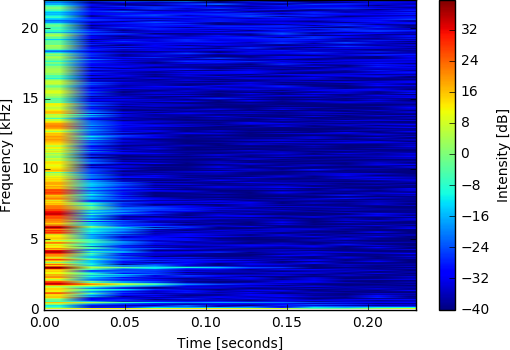
\includegraphics[width=\textwidth]{specs/spectrograms/mortarBODYLOWER_rec.png}
    \end{subfigure}%
    ~ %add desired spacing between images, e. g. ~, \quad, \qquad, \hfill etc. 
      %(or a blank line to force the subfigure onto a new line)
    \begin{subfigure}[b]{0.25\textwidth}
        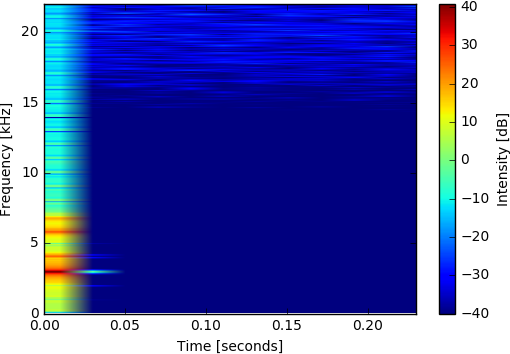
\includegraphics[width=\textwidth]{specs/spectrograms/mortarBODYLOWER_sin.png}
    \end{subfigure}%
    ~ %add desired spacing between images, e. g. ~, \quad, \qquad, \hfill etc. 
      %(or a blank line to force the subfigure onto a new line)
    \begin{subfigure}[b]{0.25\textwidth}
        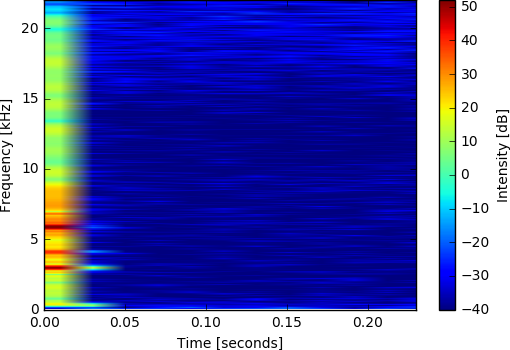
\includegraphics[width=\textwidth]{specs/spectrograms/mortarBODYLOWER_fb.png}
    \end{subfigure}%
    %add desired spacing between images, e. g. ~, \quad, \qquad, \hfill etc. 
      %(or a blank line to force the subfigure onto a new line)
      
    \begin{subfigure}[b]{0.25\textwidth}
        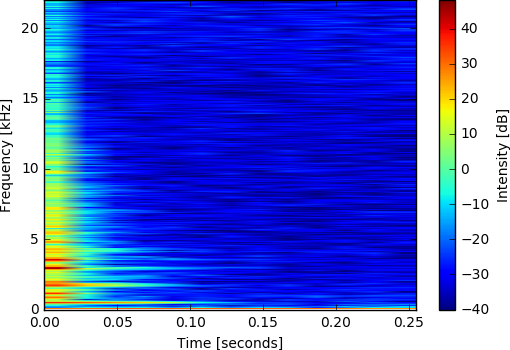
\includegraphics[width=\textwidth]{specs/spectrograms/mortarBOTTOM_rec.png}
    \end{subfigure}%
    ~ %add desired spacing between images, e. g. ~, \quad, \qquad, \hfill etc. 
      %(or a blank line to force the subfigure onto a new line)
    \begin{subfigure}[b]{0.25\textwidth}
        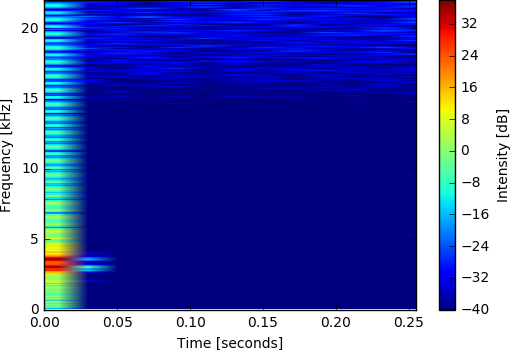
\includegraphics[width=\textwidth]{specs/spectrograms/mortarBOTTOM_sin.png}
    \end{subfigure}%
    ~ %add desired spacing between images, e. g. ~, \quad, \qquad, \hfill etc. 
      %(or a blank line to force the subfigure onto a new line)
    \begin{subfigure}[b]{0.25\textwidth}
        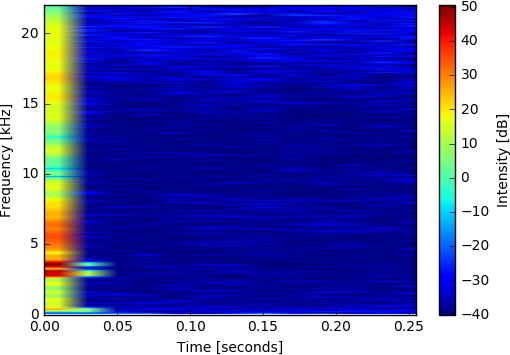
\includegraphics[width=\textwidth]{specs/spectrograms/mortarBOTTOM_fb.png}
    \end{subfigure}%
    \label{fig:spectrograms}
\end{figure}

\section*{Ceramic plate}

\begin{figure}[H]
    \centering
    \begin{subfigure}[b]{0.25\textwidth}
        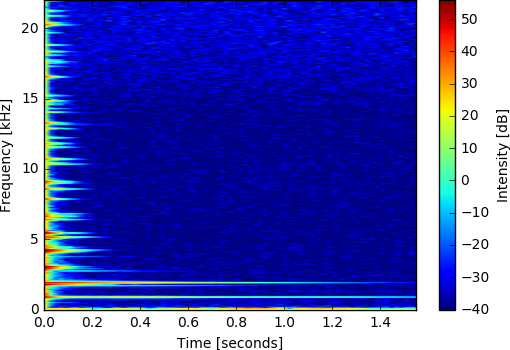
\includegraphics[width=\textwidth]{specs/spectrograms/plateOUTER_rec.png}
    \end{subfigure}%
    ~ %add desired spacing between images, e. g. ~, \quad, \qquad, \hfill etc. 
      %(or a blank line to force the subfigure onto a new line)
    \begin{subfigure}[b]{0.25\textwidth}
        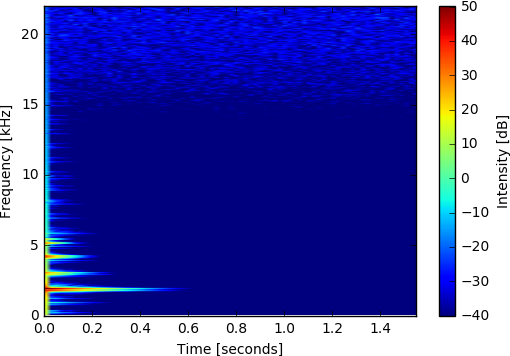
\includegraphics[width=\textwidth]{specs/spectrograms/plateOUTER_sin.png}
    \end{subfigure}%
    ~ %add desired spacing between images, e. g. ~, \quad, \qquad, \hfill etc. 
      %(or a blank line to force the subfigure onto a new line)
    \begin{subfigure}[b]{0.25\textwidth}
        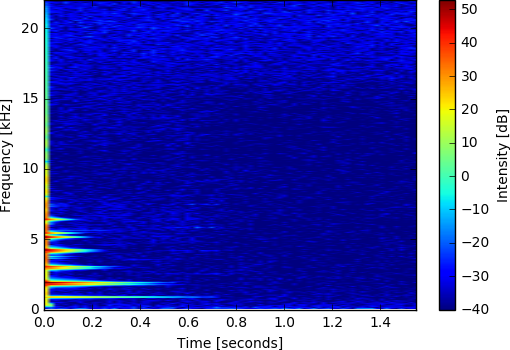
\includegraphics[width=\textwidth]{specs/spectrograms/plateOUTER_fb.png}
    \end{subfigure}%
    %add desired spacing between images, e. g. ~, \quad, \qquad, \hfill etc. 
      %(or a blank line to force the subfigure onto a new line)
      
    \begin{subfigure}[b]{0.25\textwidth}
        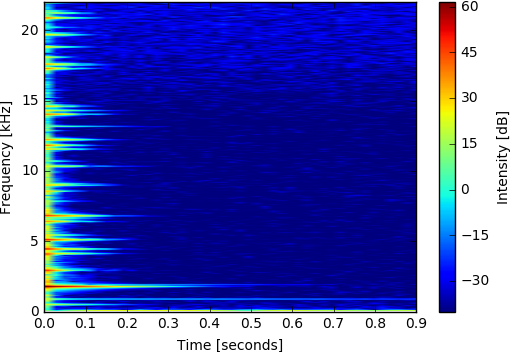
\includegraphics[width=\textwidth]{specs/spectrograms/plateMIDDLE_rec.png}
    \end{subfigure}%
    ~ %add desired spacing between images, e. g. ~, \quad, \qquad, \hfill etc. 
      %(or a blank line to force the subfigure onto a new line)
    \begin{subfigure}[b]{0.25\textwidth}
        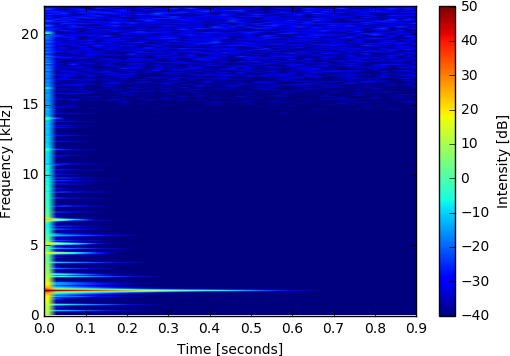
\includegraphics[width=\textwidth]{specs/spectrograms/plateMIDDLE_sin.png}
    \end{subfigure}%
    ~ %add desired spacing between images, e. g. ~, \quad, \qquad, \hfill etc. 
      %(or a blank line to force the subfigure onto a new line)
    \begin{subfigure}[b]{0.25\textwidth}
        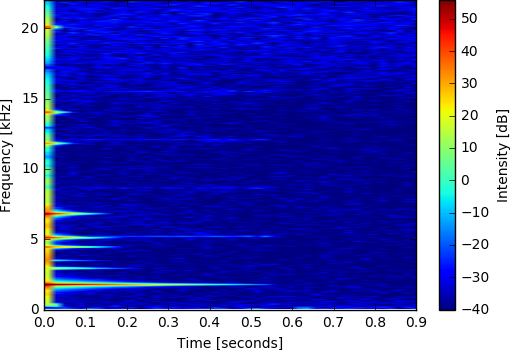
\includegraphics[width=\textwidth]{specs/spectrograms/plateMIDDLE_fb.png}
    \end{subfigure}%
    %add desired spacing between images, e. g. ~, \quad, \qquad, \hfill etc. 
      %(or a blank line to force the subfigure onto a new line)
      
    \begin{subfigure}[b]{0.25\textwidth}
        \includegraphics[width=\textwidth]{specs/spectrograms/plateCENTER_rec.png}
    \end{subfigure}%
    ~ %add desired spacing between images, e. g. ~, \quad, \qquad, \hfill etc. 
      %(or a blank line to force the subfigure onto a new line)
    \begin{subfigure}[b]{0.25\textwidth}
        \includegraphics[width=\textwidth]{specs/spectrograms/plateCENTER_sin.png}
    \end{subfigure}%
    ~ %add desired spacing between images, e. g. ~, \quad, \qquad, \hfill etc. 
      %(or a blank line to force the subfigure onto a new line)
    \begin{subfigure}[b]{0.25\textwidth}
        \includegraphics[width=\textwidth]{specs/spectrograms/plateCENTER_fb.png}
    \end{subfigure}%
\end{figure}

\section*{Wine glass}

\begin{figure}[H]
    \centering
    \begin{subfigure}[b]{0.25\textwidth}
        \includegraphics[width=\textwidth]{specs/spectrograms/wineglassTOP_rec.png}
    \end{subfigure}%
    ~ %add desired spacing between images, e. g. ~, \quad, \qquad, \hfill etc. 
      %(or a blank line to force the subfigure onto a new line)
    \begin{subfigure}[b]{0.25\textwidth}
        \includegraphics[width=\textwidth]{specs/spectrograms/wineglassTOP_sin.png}
    \end{subfigure}%
    ~ %add desired spacing between images, e. g. ~, \quad, \qquad, \hfill etc. 
      %(or a blank line to force the subfigure onto a new line)
    \begin{subfigure}[b]{0.25\textwidth}
        \includegraphics[width=\textwidth]{specs/spectrograms/wineglassTOP_fb.png}
    \end{subfigure}%
    %add desired spacing between images, e. g. ~, \quad, \qquad, \hfill etc. 
      %(or a blank line to force the subfigure onto a new line)
      
    \begin{subfigure}[b]{0.25\textwidth}
        \includegraphics[width=\textwidth]{specs/spectrograms/wineglassBODYUPPER_rec.png}
    \end{subfigure}%
    ~ %add desired spacing between images, e. g. ~, \quad, \qquad, \hfill etc. 
      %(or a blank line to force the subfigure onto a new line)
    \begin{subfigure}[b]{0.25\textwidth}
        \includegraphics[width=\textwidth]{specs/spectrograms/wineglassBODYUPPER_sin.png}
    \end{subfigure}%
    ~ %add desired spacing between images, e. g. ~, \quad, \qquad, \hfill etc. 
      %(or a blank line to force the subfigure onto a new line)
    \begin{subfigure}[b]{0.25\textwidth}
        \includegraphics[width=\textwidth]{specs/spectrograms/wineglassBODYUPPER_fb.png}
    \end{subfigure}%
    \end{figure}
    %add desired spacing between images, e. g. ~, \quad, \qquad, \hfill etc. 
      %(or a blank line to force the subfigure onto a new line)
\begin{figure}
	\centering      
    \begin{subfigure}[b]{0.25\textwidth}
        \includegraphics[width=\textwidth]{specs/spectrograms/wineglassBODYLOWER_rec.png}
    \end{subfigure}%
    ~ %add desired spacing between images, e. g. ~, \quad, \qquad, \hfill etc. 
      %(or a blank line to force the subfigure onto a new line)
    \begin{subfigure}[b]{0.25\textwidth}
        \includegraphics[width=\textwidth]{specs/spectrograms/wineglassBODYLOWER_sin.png}
    \end{subfigure}%
    ~ %add desired spacing between images, e. g. ~, \quad, \qquad, \hfill etc. 
      %(or a blank line to force the subfigure onto a new line)
    \begin{subfigure}[b]{0.25\textwidth}
        \includegraphics[width=\textwidth]{specs/spectrograms/wineglassBODYLOWER_fb.png}
    \end{subfigure}%
    %add desired spacing between images, e. g. ~, \quad, \qquad, \hfill etc. 
      %(or a blank line to force the subfigure onto a new line)
      
    \begin{subfigure}[b]{0.25\textwidth}
        \includegraphics[width=\textwidth]{specs/spectrograms/wineglassSTEM_rec.png}
    \end{subfigure}%
    ~ %add desired spacing between images, e. g. ~, \quad, \qquad, \hfill etc. 
      %(or a blank line to force the subfigure onto a new line)
    \begin{subfigure}[b]{0.25\textwidth}
        \includegraphics[width=\textwidth]{specs/spectrograms/wineglassSTEM_sin.png}
    \end{subfigure}%
    ~ %add desired spacing between images, e. g. ~, \quad, \qquad, \hfill etc. 
      %(or a blank line to force the subfigure onto a new line)
    \begin{subfigure}[b]{0.25\textwidth}
        \includegraphics[width=\textwidth]{specs/spectrograms/wineglassSTEM_fb.png}
    \end{subfigure}%
    %add desired spacing between images, e. g. ~, \quad, \qquad, \hfill etc. 
      %(or a blank line to force the subfigure onto a new line)
      
    \begin{subfigure}[b]{0.25\textwidth}
        \includegraphics[width=\textwidth]{specs/spectrograms/wineglassFOOT_rec.png}
    \end{subfigure}%
    ~ %add desired spacing between images, e. g. ~, \quad, \qquad, \hfill etc. 
      %(or a blank line to force the subfigure onto a new line)
    \begin{subfigure}[b]{0.25\textwidth}
        \includegraphics[width=\textwidth]{specs/spectrograms/wineglassFOOT_sin.png}
    \end{subfigure}%
    ~ %add desired spacing between images, e. g. ~, \quad, \qquad, \hfill etc. 
      %(or a blank line to force the subfigure onto a new line)
    \begin{subfigure}[b]{0.25\textwidth}
        \includegraphics[width=\textwidth]{specs/spectrograms/wineglassFOOT_fb.png}
    \end{subfigure}%
\end{figure}

\section*{Metallic wok}

\begin{figure}[H]
    \centering
    \begin{subfigure}[b]{0.25\textwidth}
        \includegraphics[width=\textwidth]{specs/spectrograms/wokBODYUPPER_rec.png}
    \end{subfigure}%
    ~ %add desired spacing between images, e. g. ~, \quad, \qquad, \hfill etc. 
      %(or a blank line to force the subfigure onto a new line)
    \begin{subfigure}[b]{0.25\textwidth}
        \includegraphics[width=\textwidth]{specs/spectrograms/wokBODYUPPER_sin.png}
    \end{subfigure}%
    ~ %add desired spacing between images, e. g. ~, \quad, \qquad, \hfill etc. 
      %(or a blank line to force the subfigure onto a new line)
    \begin{subfigure}[b]{0.25\textwidth}
        \includegraphics[width=\textwidth]{specs/spectrograms/wokBODYUPPER_fb.png}
    \end{subfigure}%
    %add desired spacing between images, e. g. ~, \quad, \qquad, \hfill etc. 
      %(or a blank line to force the subfigure onto a new line)
      
    \begin{subfigure}[b]{0.25\textwidth}
        \includegraphics[width=\textwidth]{specs/spectrograms/wokBODYLOWER_rec.png}
    \end{subfigure}%
    ~ %add desired spacing between images, e. g. ~, \quad, \qquad, \hfill etc. 
      %(or a blank line to force the subfigure onto a new line)
    \begin{subfigure}[b]{0.25\textwidth}
        \includegraphics[width=\textwidth]{specs/spectrograms/wokBODYLOWER_sin.png}
    \end{subfigure}%
    ~ %add desired spacing between images, e. g. ~, \quad, \qquad, \hfill etc. 
      %(or a blank line to force the subfigure onto a new line)
    \begin{subfigure}[b]{0.25\textwidth}
        \includegraphics[width=\textwidth]{specs/spectrograms/wokBODYLOWER_fb.png}
    \end{subfigure}%
    %add desired spacing between images, e. g. ~, \quad, \qquad, \hfill etc. 
      %(or a blank line to force the subfigure onto a new line)

    \begin{subfigure}[b]{0.25\textwidth}
        \includegraphics[width=\textwidth]{specs/spectrograms/wokBOTTOMEDGE_rec.png}
    \end{subfigure}%
    ~ %add desired spacing between images, e. g. ~, \quad, \qquad, \hfill etc. 
      %(or a blank line to force the subfigure onto a new line)
    \begin{subfigure}[b]{0.25\textwidth}
        \includegraphics[width=\textwidth]{specs/spectrograms/wokBOTTOMEDGE_sin.png}
    \end{subfigure}%
     ~ %add desired spacing between images, e. g. ~, \quad, \qquad, \hfill etc. 
      %(or a blank line to force the subfigure onto a new line)
    \begin{subfigure}[b]{0.25\textwidth}
        \includegraphics[width=\textwidth]{specs/spectrograms/wokBOTTOMEDGE_fb.png}
    \end{subfigure}%
    %add desired spacing between images, e. g. ~, \quad, \qquad, \hfill etc. 
      %(or a blank line to force the subfigure onto a new line)
      
    \begin{subfigure}[b]{0.25\textwidth}
        \includegraphics[width=\textwidth]{specs/spectrograms/wokBOTTOMMIDDLE_rec.png}
    \end{subfigure}%
    ~ %add desired spacing between images, e. g. ~, \quad, \qquad, \hfill etc. 
      %(or a blank line to force the subfigure onto a new line)
    \begin{subfigure}[b]{0.25\textwidth}
        \includegraphics[width=\textwidth]{specs/spectrograms/wokBOTTOMMIDDLE_sin.png}
    \end{subfigure}%
    ~ %add desired spacing between images, e. g. ~, \quad, \qquad, \hfill etc. 
      %(or a blank line to force the subfigure onto a new line)
    \begin{subfigure}[b]{0.25\textwidth}
        \includegraphics[width=\textwidth]{specs/spectrograms/wokBOTTOMMIDDLE_fb.png}
    \end{subfigure}%
\end{figure}


\chapter{User Guide to our product}\label{ap:guide}

\begin{itemize}
\item Record impact sounds
\item Put audio files into the data extraction algorithm
\item Take the output data and put them into unity
\item Make an FBX\textsuperscript{\textregistered} model of your object with the same dimensions and put it into a Unity\textsuperscript{\textregistered} scene as game object
\item Assign the audio manager to the game object
\item Tag the game object with the corresponding tag
\item Adjust the material, size and object roughness sliders
\end{itemize}



% \backmatter % for glossary, index, back page
\end{document}
